\Section{Signal Modifier Parameter Inference with cINNs}

In this chapter, the performance of the network will be characterized in detail. Two network setups will be considered: one without and one with a summary network reducing the representation of the conditions. These networks will be referred to as cINN and SN-cINN (for summary network-extended cINN). It will be shown that the setup without a summary network results in superior performance. 

\Subsection{Training Performance}

The loss functions for both trainings are shown in fig. \ref{fig:losses} for the different setups. The location of the models with the lowest validation loss is indicated by the red dashed line. It is visible the SN-cINN models suffer from overtraining -- no network from the three independent runs with different initializations has converged during training. This effect has also been observed in \cite{Ksoll_2020}. The structure of the summary network is optimized so that this network model achieves the lowest validation loss; models with a deeper summary network or less output nodes are observed to produce worse results with a higher loss.

\begin{figure}[h!]
	\begin{minipage}{.5\textwidth}
		\centering
		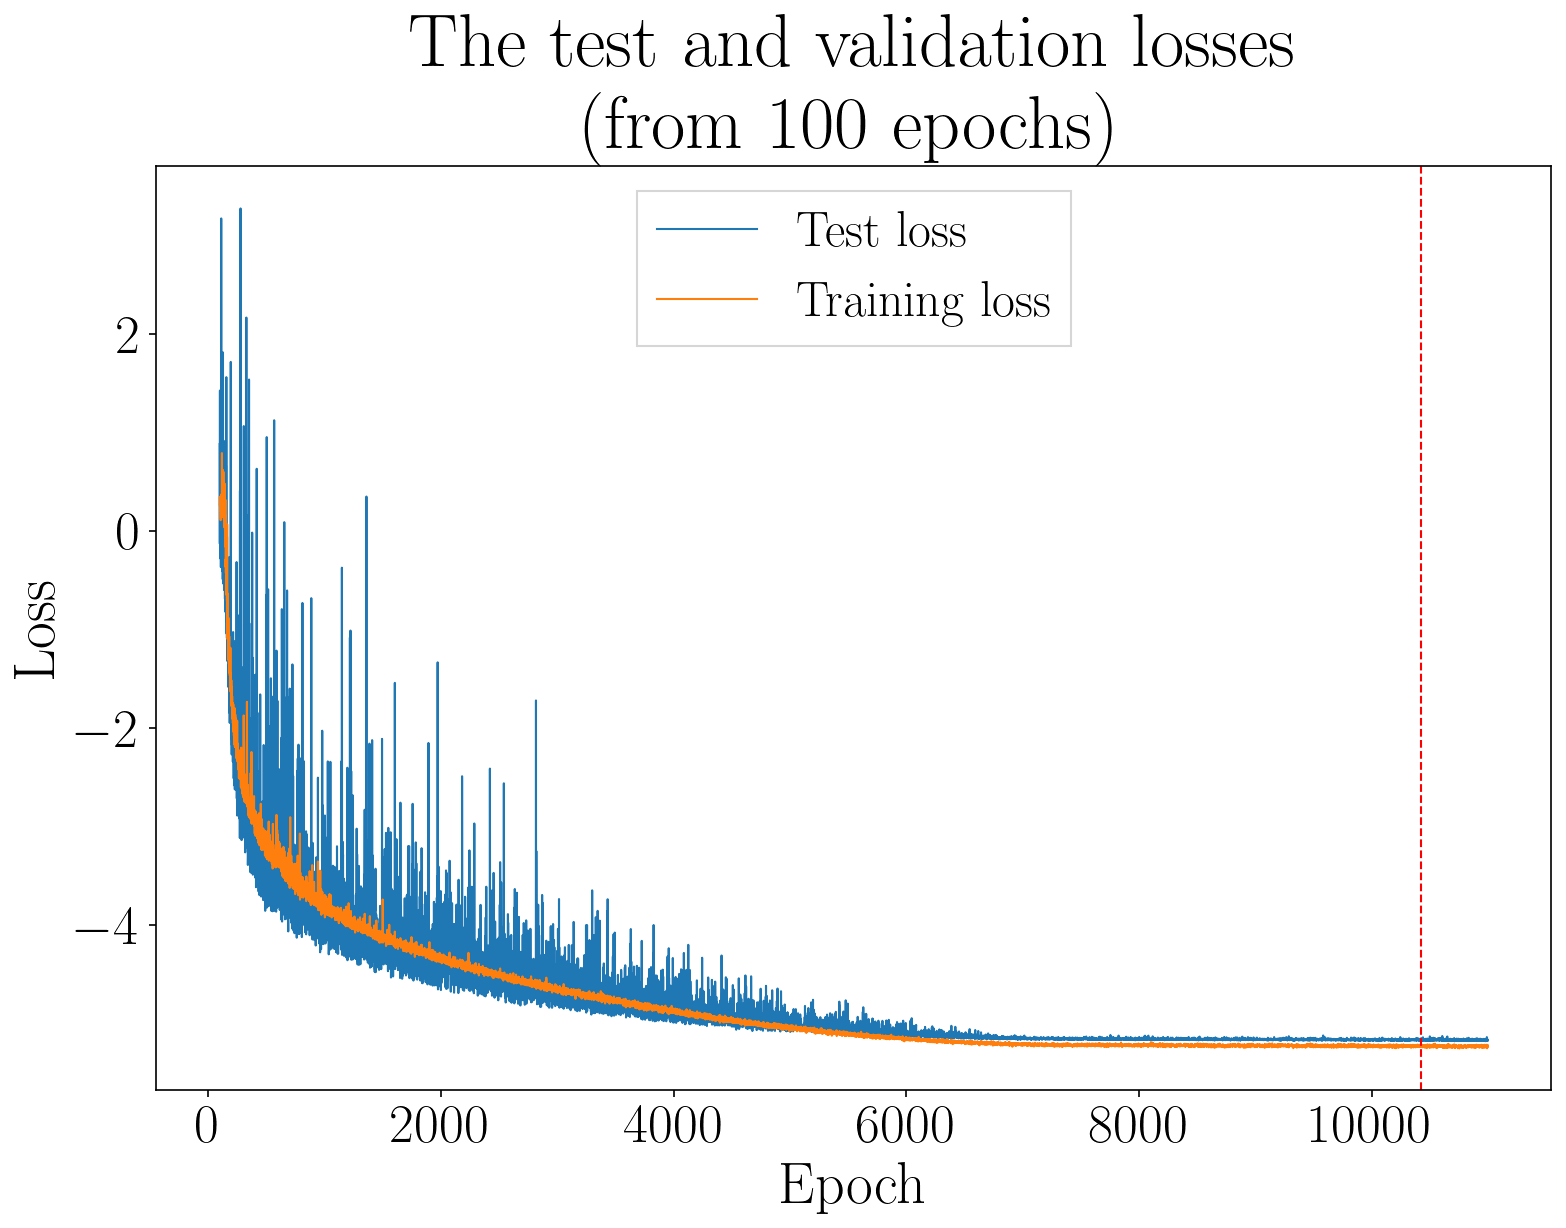
\includegraphics[width=\linewidth]{figures/inference/losses}
	\end{minipage}%
	\begin{minipage}{.5\textwidth}
		\centering
		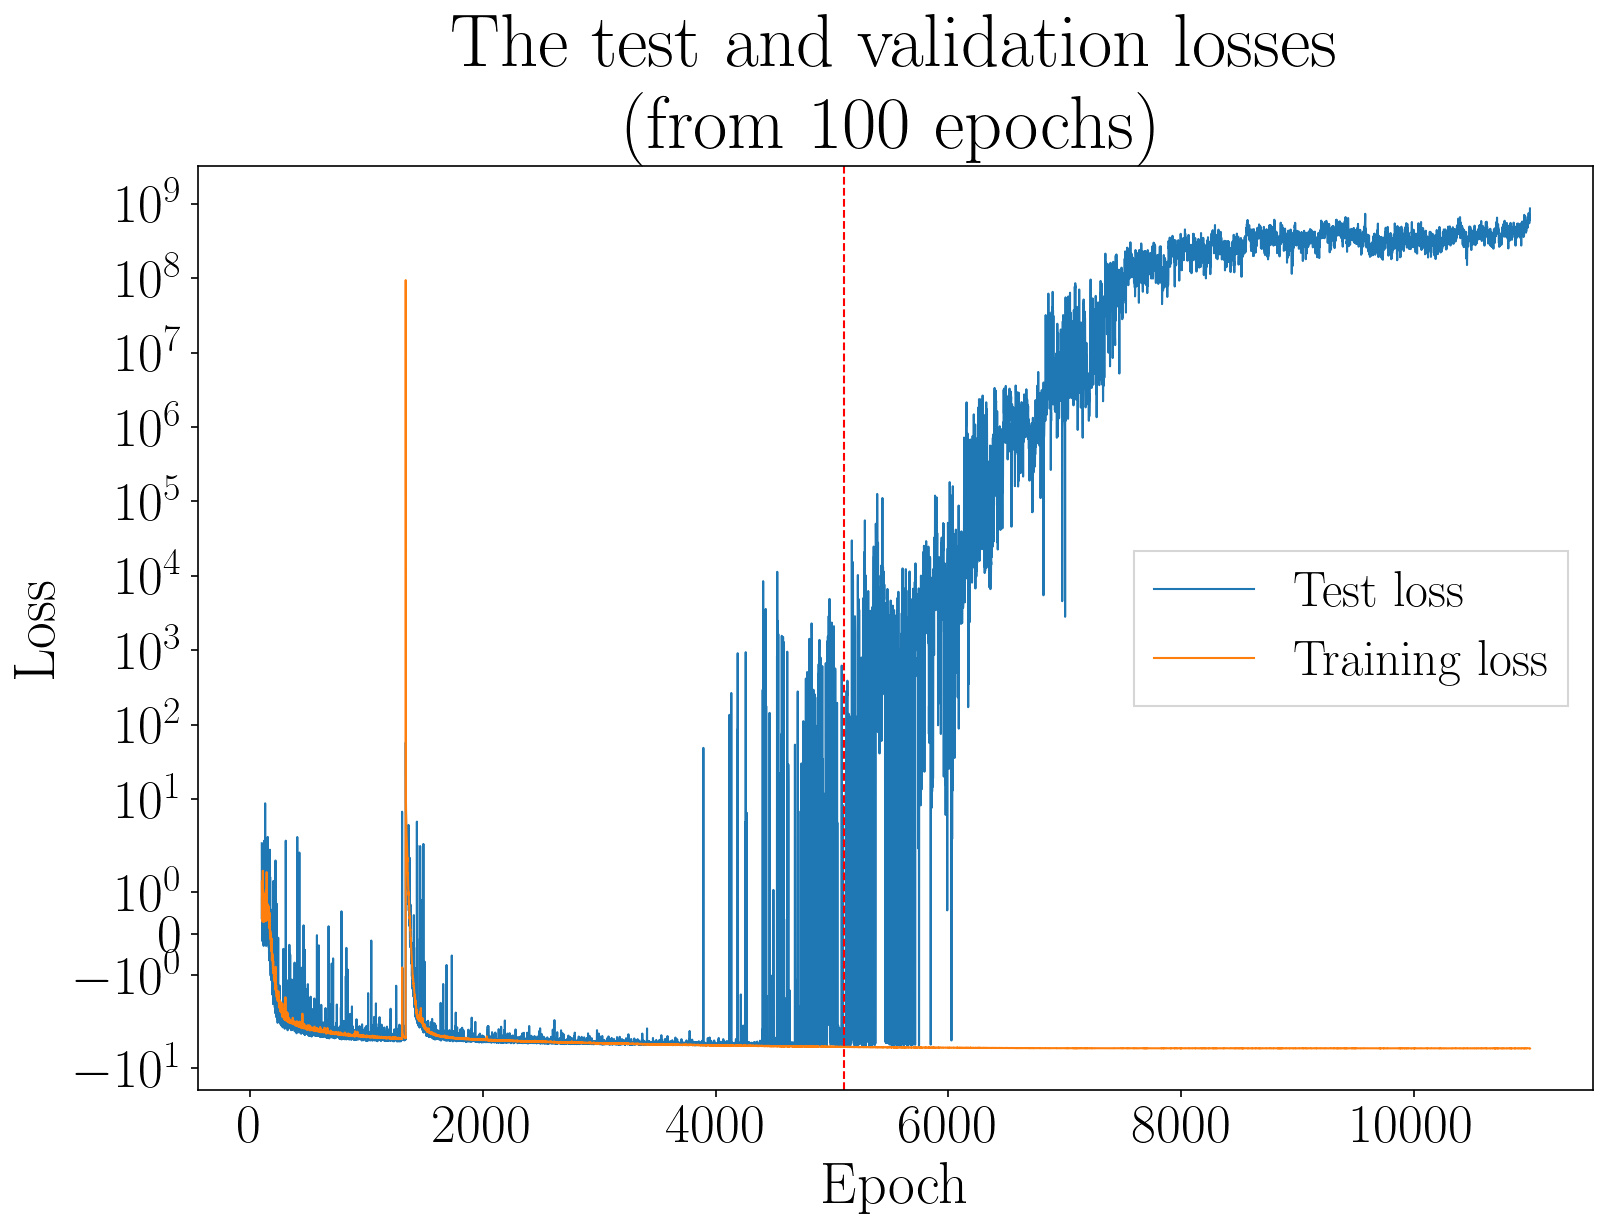
\includegraphics[width=\linewidth]{figures/inference/losses_SN}
	\end{minipage}
	\centering
	\caption{The loss values for each network from the 100th epoch for the cINN (left) and for the SN-cINN (right). Initial losses are removed as they disturb the graph. Models with the lowest validation loss are shown with the red dashed line. The corresponding loss values are $-5.16$ for the cINN and $-4.96$ for the SN-cINN. Overtraining can be observed for the summary network after 4000 epochs, where the loss values explode.}
	\label{fig:losses}
\end{figure}

The strongly fluctuating and exploding test loss for the SN-cINN indicates that a reduction of the conditions does not result in a better generalisation capability of the model, but only lowers the training loss with an overtraining effect. Thus, the representation of the conditions is already well chosen and the reduction of the conditions necessarily result in performances of lower quality.

\Subsection{Latent Space Distributions}

At the end of ch. \ref{ch:deeplearning}, the loss function has been constructed in a way that the input variables are mapped to a multivariate normal distribution with $\mu = 0$ and $\Sigma=\mathds{1}$. Loss functions alone with their singular numeric value are hard to interpret in terms of the quality of the resulting mapping. To examine whether there are any issues with the setup, the shape of the latent space distribution serves as a suitable candidate.

The latent space distributions for both networks are shown in fig. \ref{fig:latents} for the models with the lowest test loss. The distribution of the network outputs are shown in the blue histograms while a normal function with mean 0 and standard deviation 1 is shown in red.

\begin{figure}[h!]
	\centering
	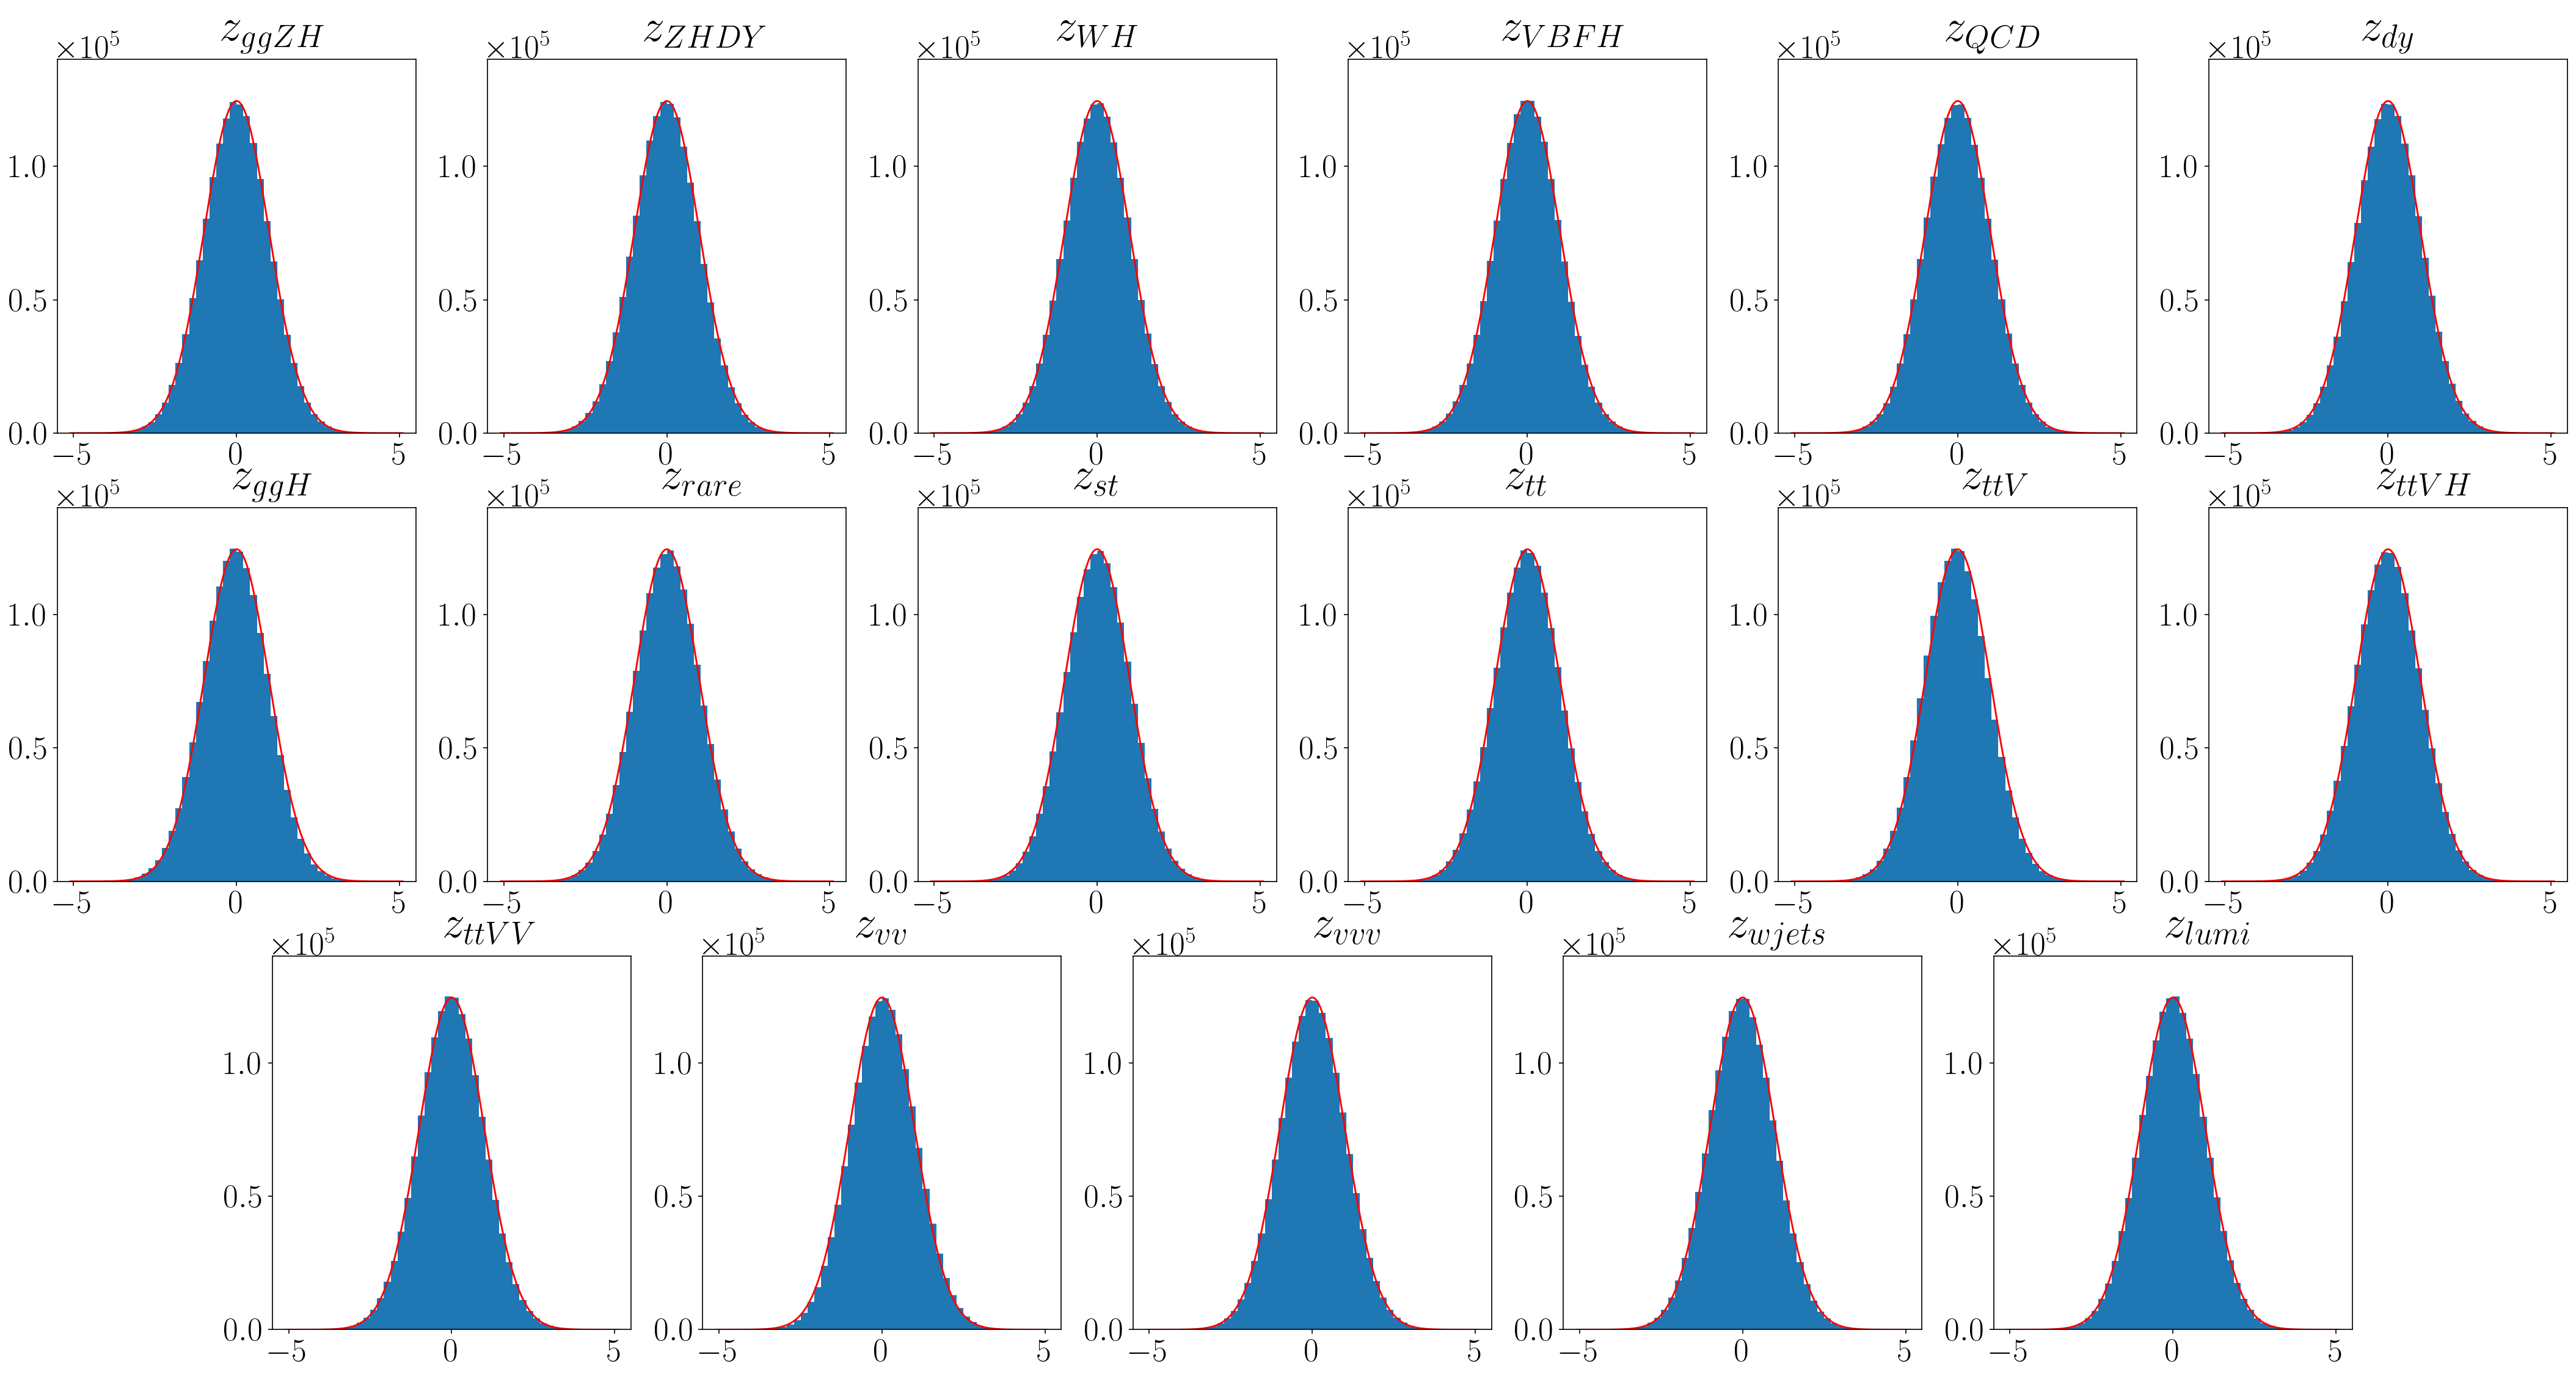
\includegraphics[width=\textwidth]{figures/inference/ls.png}
	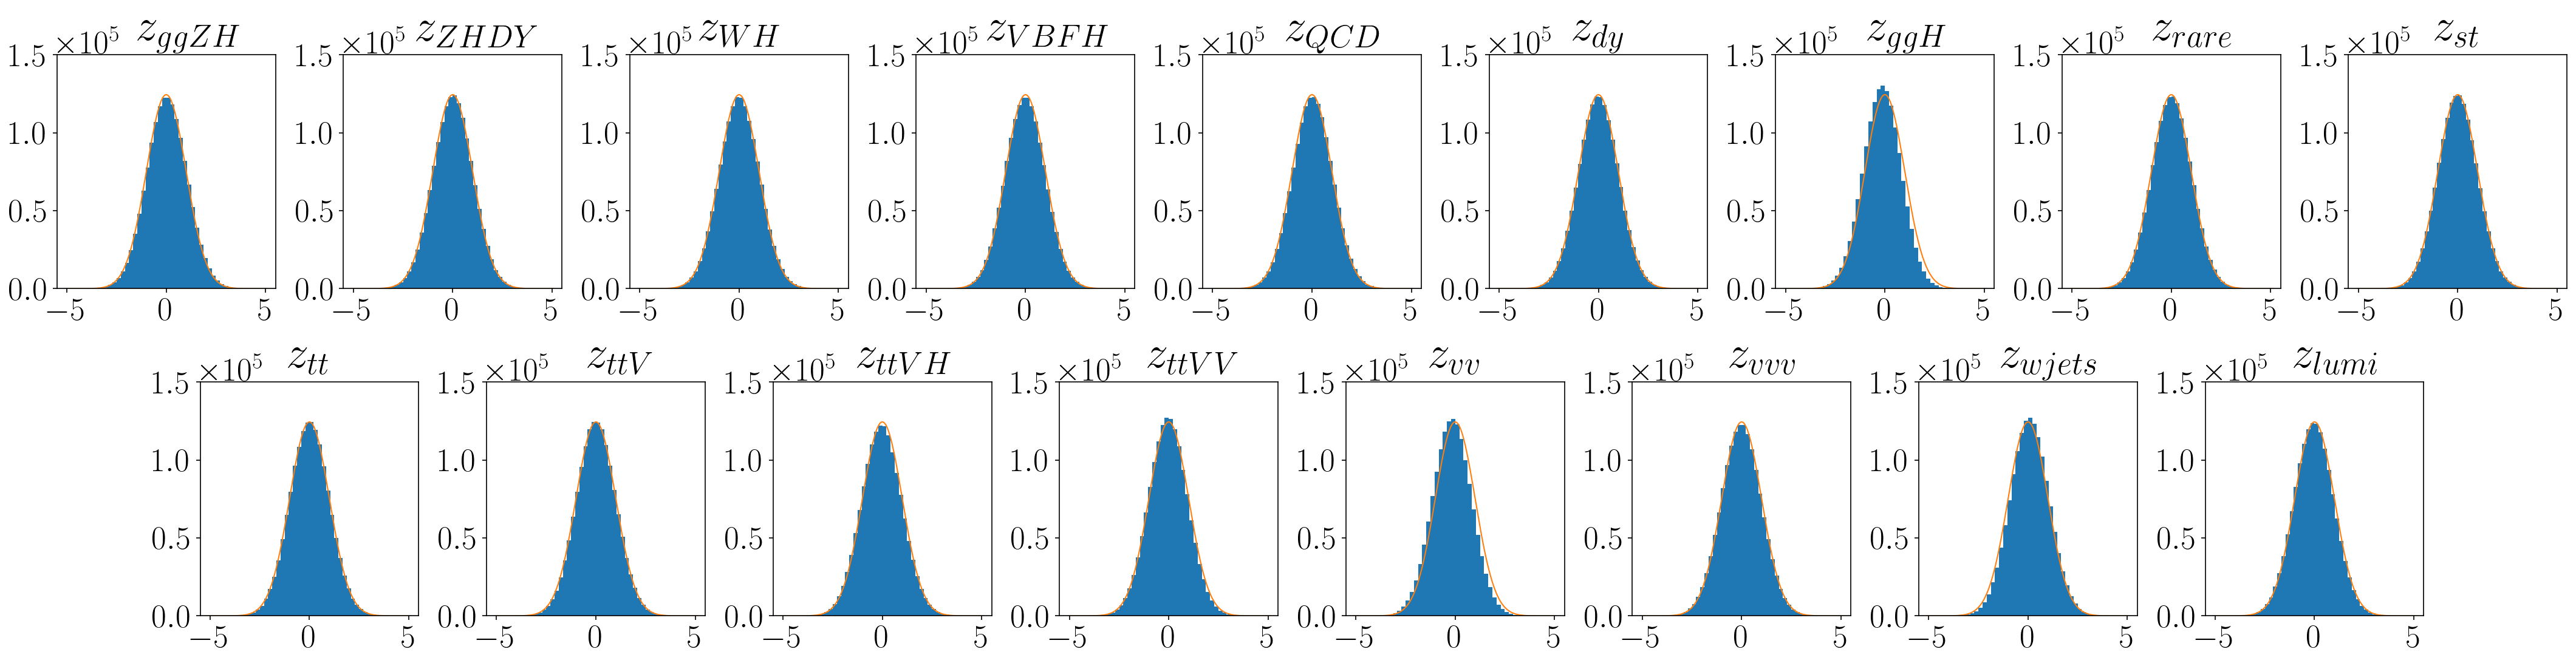
\includegraphics[width=\textwidth]{figures/inference/ls_SN.png}
	\caption{Latent space distribution for the cINN without (top) and with (bottom) a summary network.}
	\label{fig:latents}
\end{figure}

All of the above distributions in blue are well-described by the orange curve for both networks. The network thus manages to map the input distributions to $\mathcal{N}(z; 0,1)$ well enough. The question now remains how well the cINN is capable of producing the posteriors.

\Subsection{Calibration Curves}

A measure of evaluating the quality of the produced posteriors are the calibration errors. The calibration error for a given quantile (i.e. $q\in [0, 1]$) is defined for all histograms $N$ as

\begin{equation*}
	e_{cal}(q) = \frac{N^q_{in}}{N} - q
\end{equation*}

where $N^q_{in}$ is the number of histograms containing the true value within their $q$ quantile. For ideal posteriors, this measure is 0 for all quantiles $q$; any deviations from that signals the presence of biases and of hidden correlations within the network. Naturally, no network can reproduce the ideal results, as the global optimum can only be approximated. For all quantiles, the ratio of histograms containing the true value in their $q$ quantile as a function of $q$ is shown in fig. \ref{fig:ecals}.

\begin{figure}[h!]
	\centering
	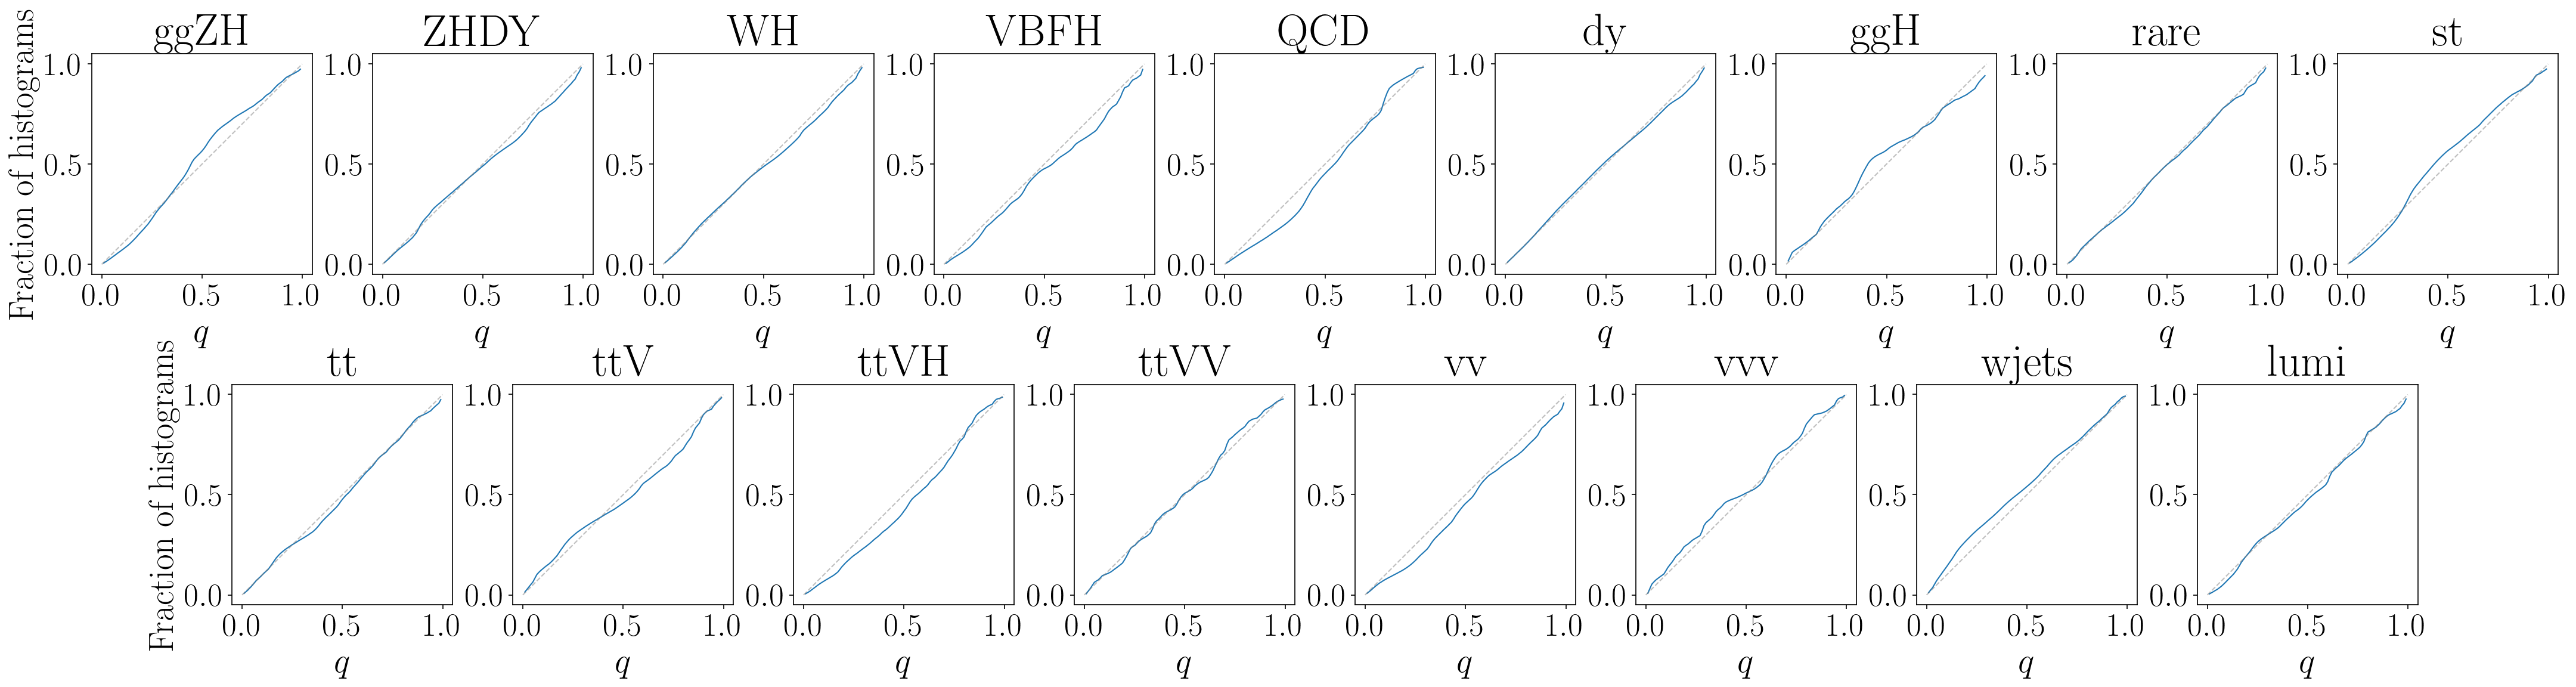
\includegraphics[width=\linewidth]{figures/inference/ecal}
	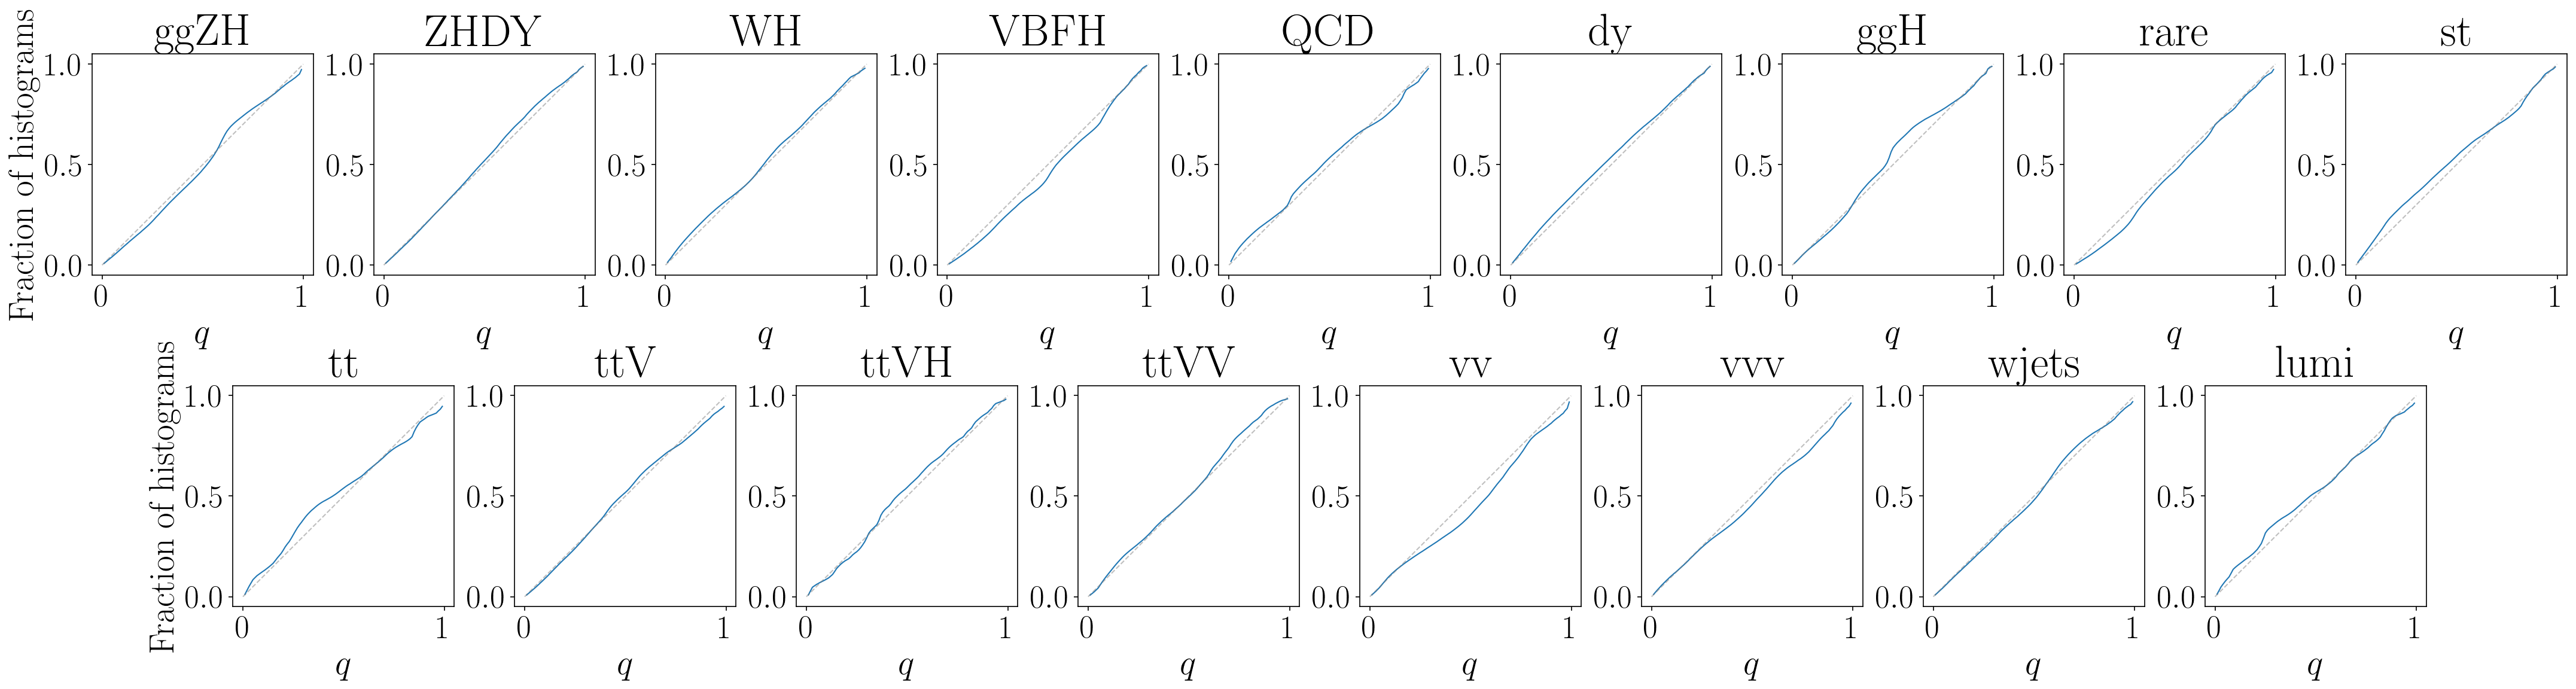
\includegraphics[width=\linewidth]{figures/inference/ecal_SN}
	\caption{The calibration curves for the cINN and summary network-extended cINN. Note the closeness to the perfect calibration curve shown in the gray dashed line.}
	\label{fig:ecals}
\end{figure}

One way to describe how strong these biases are in the network is the median calibration error, defined as

\begin{equation*}
	e^{med}_{cal} = \underset{q}{\text{med}} \left|\frac{N^q_{in}}{N} - q\right|.
\end{equation*}

It describes the median absolute distance of the histogram ratios to the ideal case. These values for both networks have been listed in tab. \ref{tab:ecal_med}. As it can be seen from the table all of these values are $e^{med}_{cal}\lesssim\mathcal{O}(0.04)$. With such small mean deviations and calibration curves being close to the perfect calibration line, the resulting network model has no significant inherent biases due to wrong initialization or other nontrivial effects.

\begin{table}[h!]
	\centering
	\begin{tabular}{ccc}
		\multirow{2}{*}{Process}& \multicolumn{2}{c}{$e^{med}_{cal}$} \\
		 & cINN & SN-cINN \\
		\hline
		\texttt{ggZH }   & 0.0156    &    0.0258  \\
		\texttt{ZHDY }   & 0.0299    &    0.0103  \\
		\texttt{WH   }   & 0.0148    &    0.0176  \\
		\texttt{VBFH }   & 0.0256    &    0.0428  \\
		\texttt{QCD  }   & 0.0147    &    0.0285  \\
		\texttt{dy   }   & 0.0133    &    0.0323  \\
		\texttt{ggH  }   & 0.0395    &    0.0183  \\
		\texttt{rare }   & 0.0399    &    0.0261  \\
		\texttt{st   }   & 0.0229    &    0.0323  \\
		\texttt{tt   }   & 0.0101    &    0.0300  \\
		\texttt{ttV  }   & 0.0212    &    0.0144  \\
		\texttt{ttVH }   & 0.0159    &    0.0227  \\
		\texttt{ttVV }   & 0.0403    &    0.0146  \\
		\texttt{vv   }   & 0.0333    &    0.0441  \\
		\texttt{vvv  }   & 0.0326    &    0.0331  \\
		\texttt{wjets}   & 0.0070    &    0.0127  \\
		\texttt{lumi }   & 0.0156    &    0.0248  \\
		\hline
	\end{tabular}
	\caption{The median calibration errors for the cINN and the summary network-extended (SN-cINN).}
	\label{tab:ecal_med}
\end{table}

\Subsection{Network Predictions}

The predictions for the complete test dataset are shown in fig. \ref{fig:predictions}. For each two dimensional histogram, the x axis shows the predicted values for a parameter on the y axis. In these plots several structures are clearly visible, which can be categorised into three groups for both networks:

\begin{itemize}
	\item[] \textit{Unrecognized processes} are those, where the network has difficulties obtaining the parameter with which the processes had been scaled. These are \texttt{VBFH, ggH, ttVH, ttVV, vvv} which are rare background processes. Due to the network not being able to differentiate between the different scalings, all of these are fitted close to the mean of the prior distribution, resulting in the thin vertical distribution in fig. \ref{fig:predictions}. Their contribution to each bin in the conditions is shown in fig. \ref{fig:cond_without_sig_bkg} in orange. From the distribution even without signal and main background processes, their contribution is extremely low.
	
	\begin{figure}[h!]
		\centering
		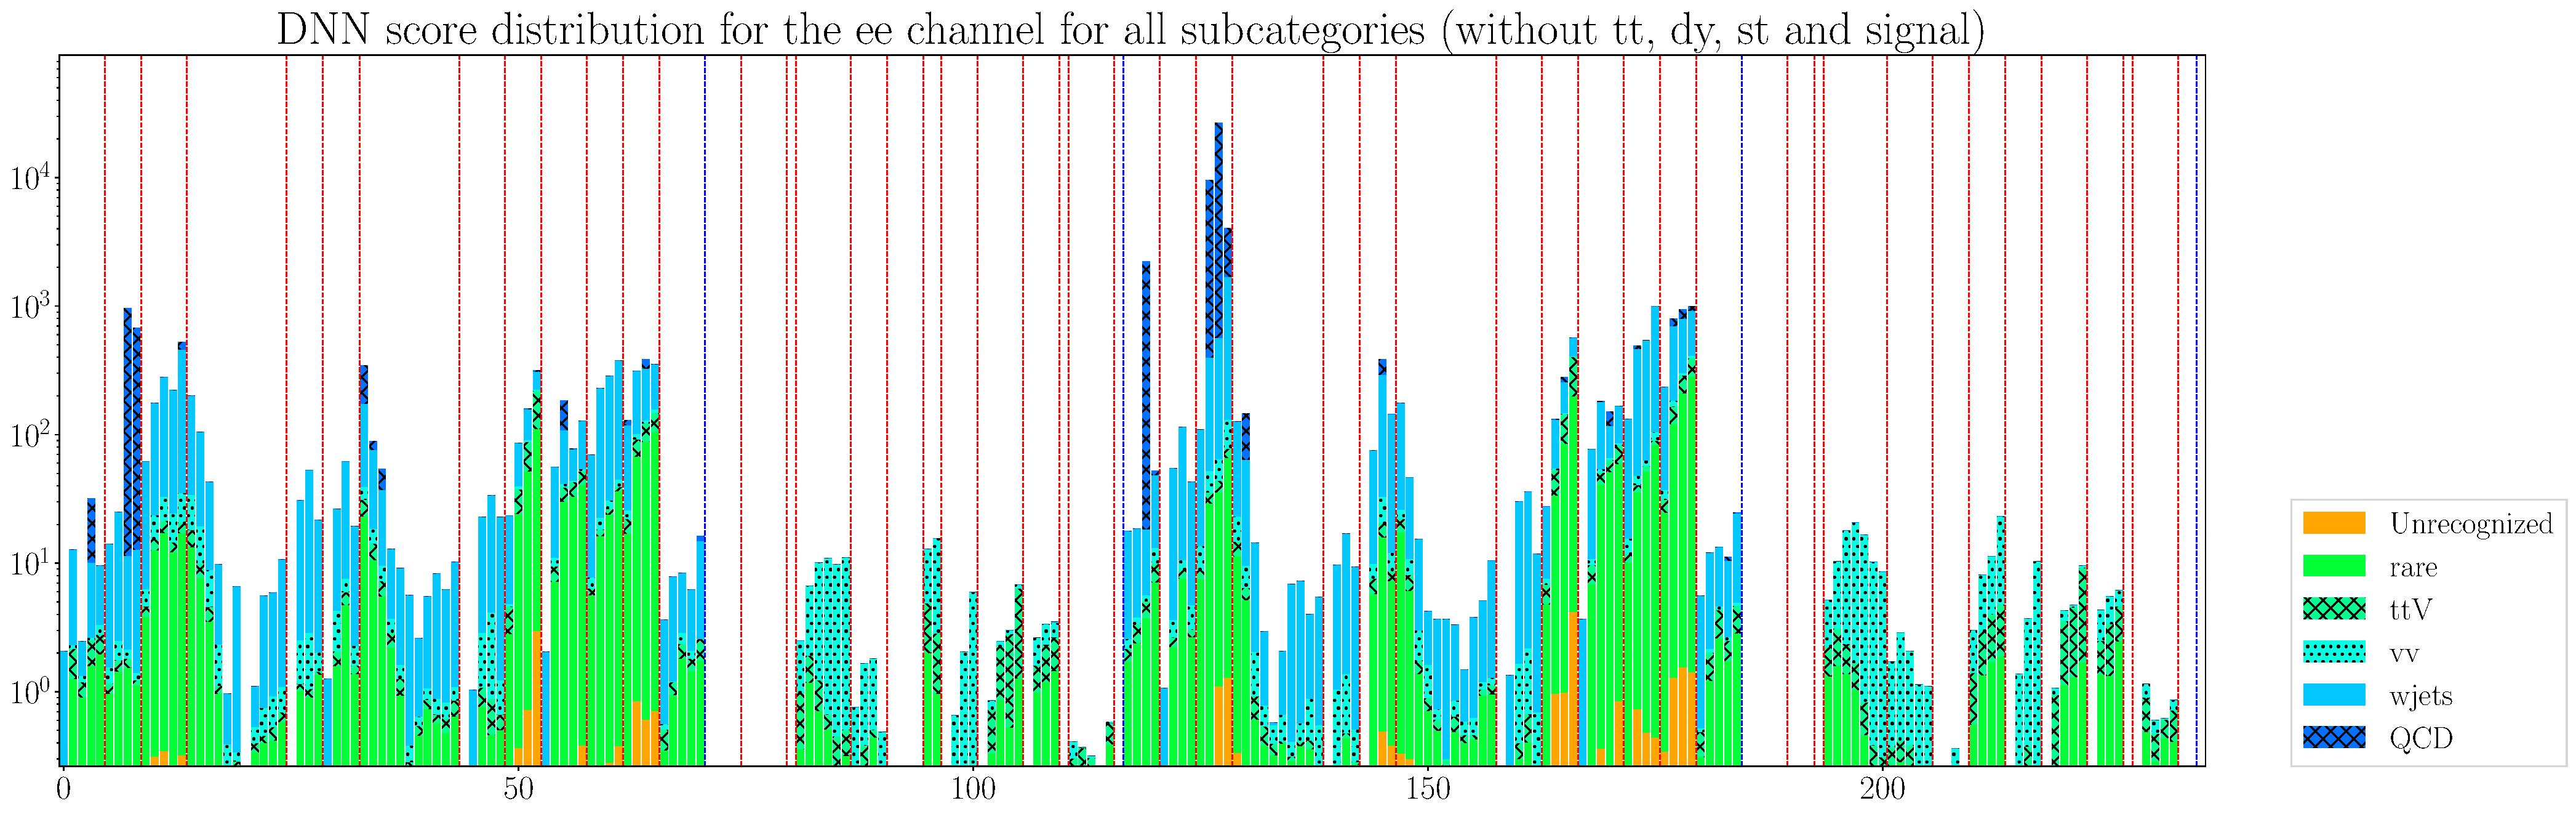
\includegraphics[width=\linewidth]{figures/inference/cond4_sorted_no_main_bkg_no_sig.pdf}
		\caption{Nominal conditions sorted by relative process occurrence without main background \texttt{tt, dy, st} and signal processes, showing the total contribution of the unrecognized processes in orange. Note that the content of each orange bin is $\lesssim\mathcal{O}(\sqrt{N})$, so their contribution is suppressed by statistical effects -- even without main background and signal processes.}
		\label{fig:cond_without_sig_bkg}
	\end{figure}
	
	\item[] \textit{Weakly recognized processes} are \texttt{rare}, \texttt{ttV}, \texttt{vv}. For these processes, the network can already resolve sevaral parameters close to the mean, from where the sensitivity starts to develop during training. Parameters further away from the mean are still fit the average value, resulting in an overall lense-like shape.
	\item[] \textit{Recognized processes} are all signal processes \texttt{ggZH}, \texttt{ZHDY} and \texttt{WH} and the major background sources \texttt{QCD}, \texttt{dy}, \texttt{st}, \texttt{tt}, \texttt{wjets}. For these processes, most modifier parameters predictions lie close to the true parameter value, hence distribution scatter around the perfect prediction diagonal.
\end{itemize}

For the signal processes \texttt{ggZH}, \texttt{ZHDY} and \texttt{WH} a decrease in sensitivity for $\mu\lesssim10$ resulting in a tail-like structure stretching towards the mean has been observed. Since their contribution is already low, the added statistical and systematic effects renders these statistically undetectable. The most significant of these effects is the Poisson bin-variation, as it modifies all bins with $\sqrt{N}$.

As the calibration curves show no signs of inherent biases in the resulting model, broader posterior distributions in in this range are expected. This will be discussed in the next section.

In general, this resolution effect only be can further tackled by a more refined event selection and/or categorization, which can help to further reduce background or even increase the signal yield. The discussion of these techniques however lies beyond the scope of this thesis.

\begin{figure}[h!]
	\centering
	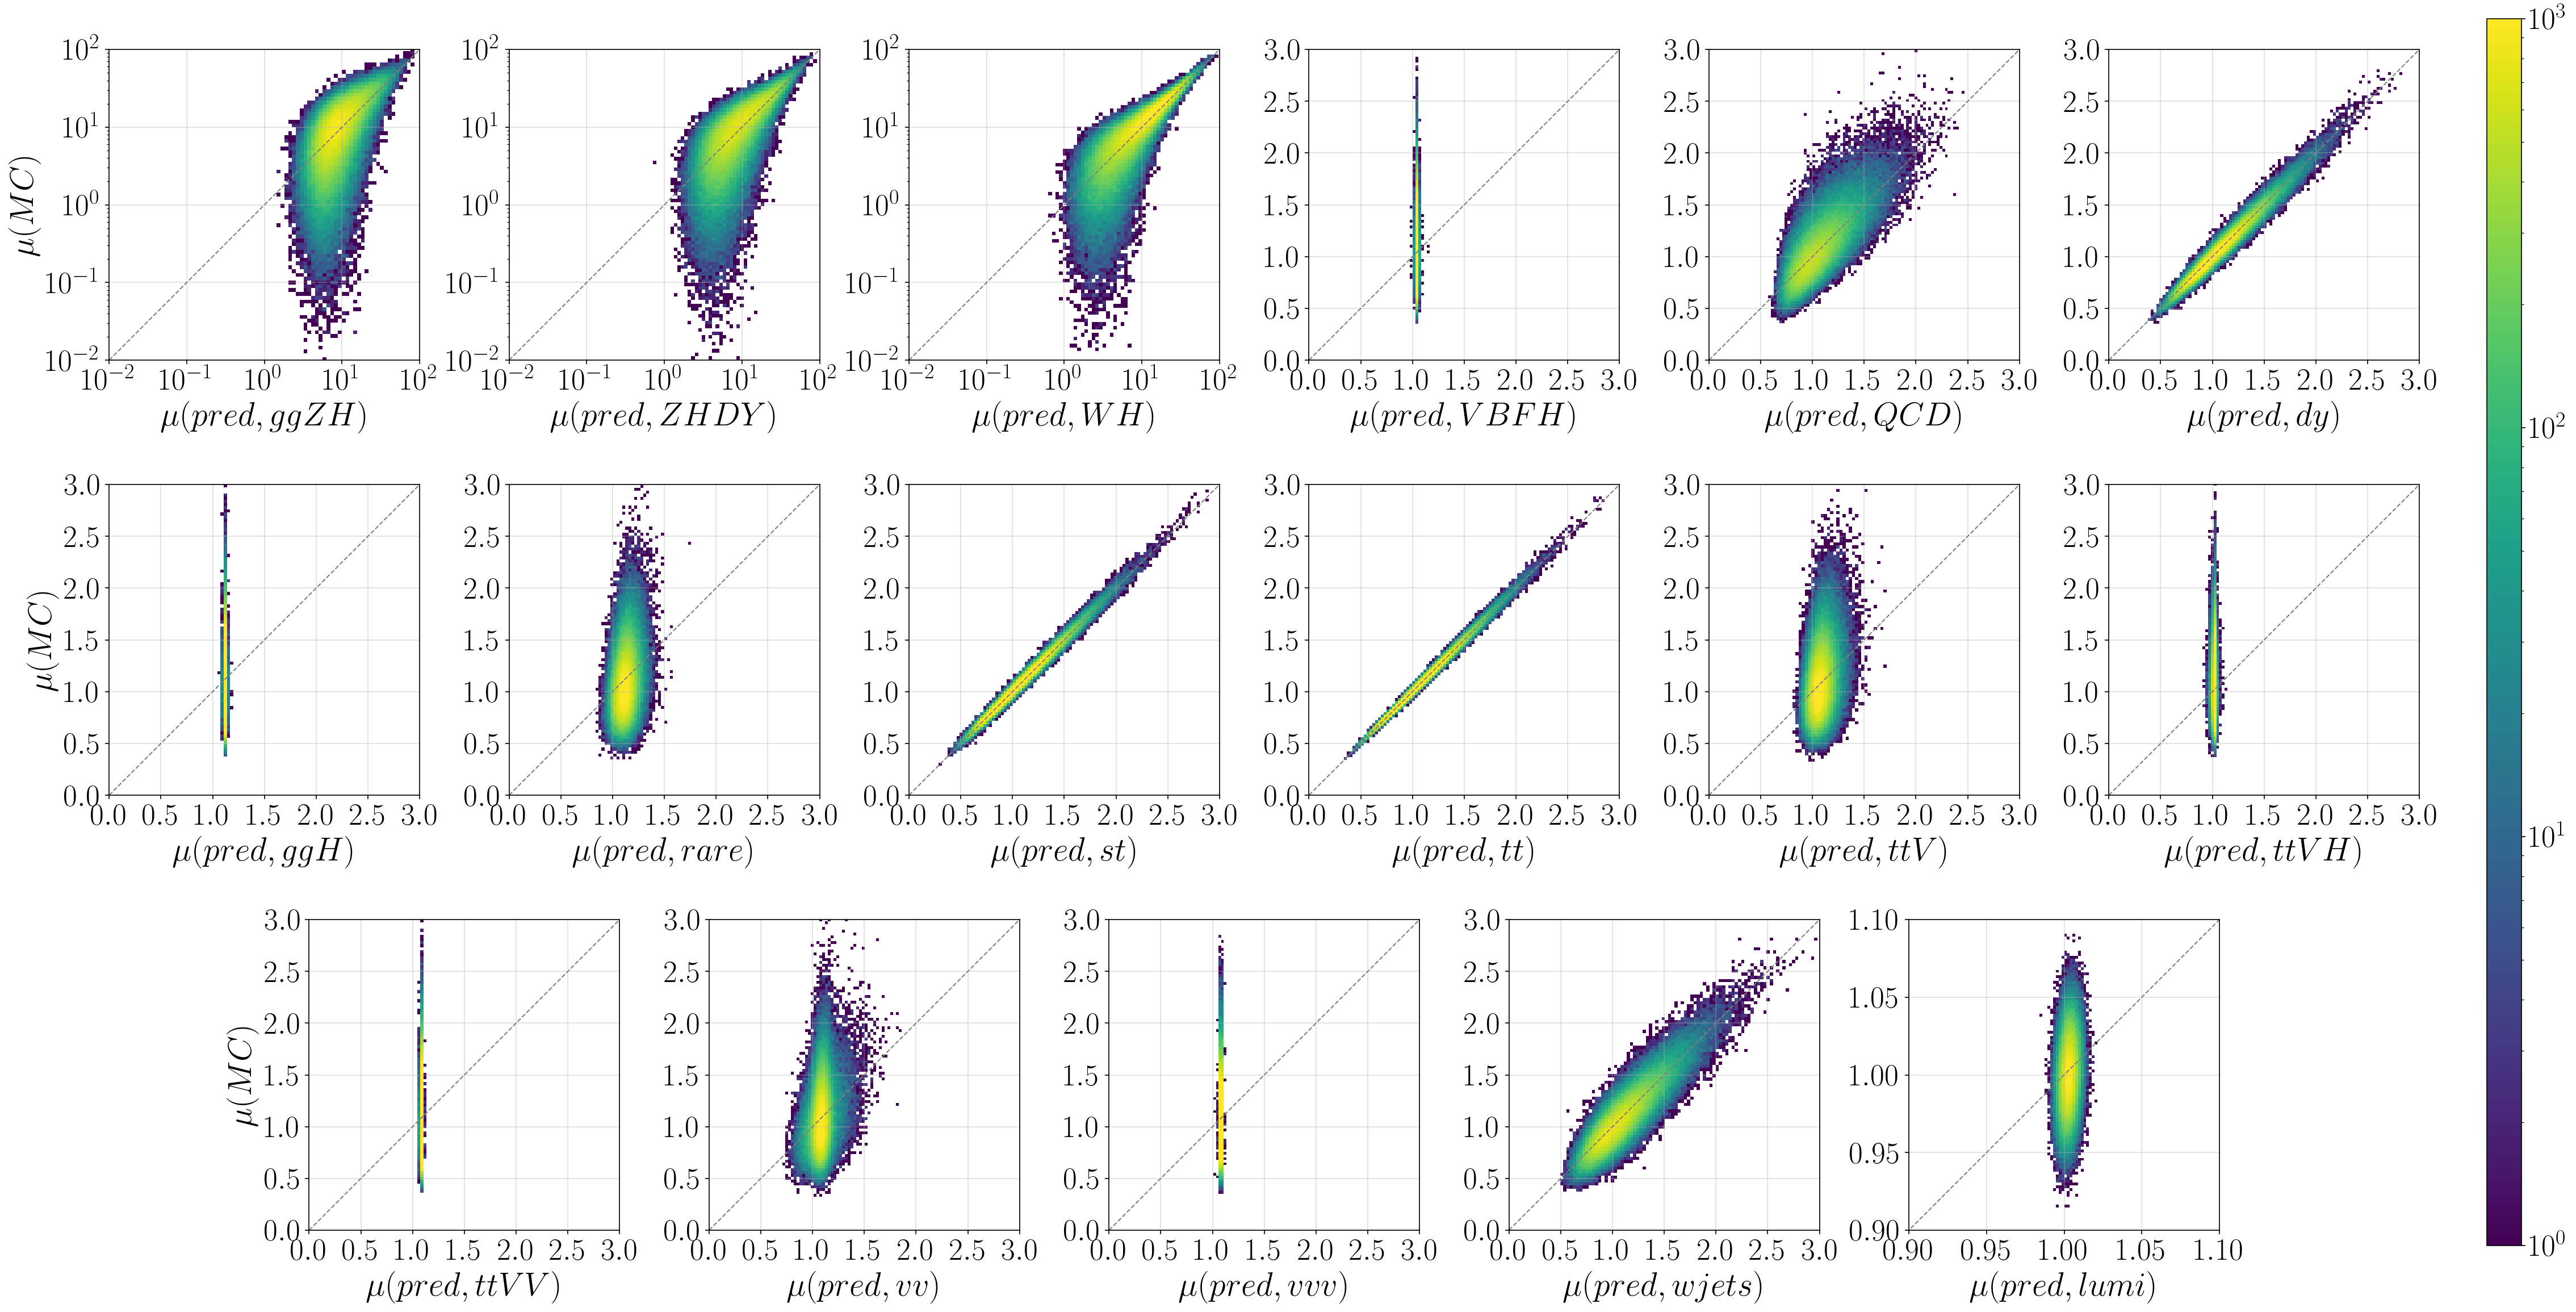
\includegraphics[width=\linewidth]{figures/inference/p}
	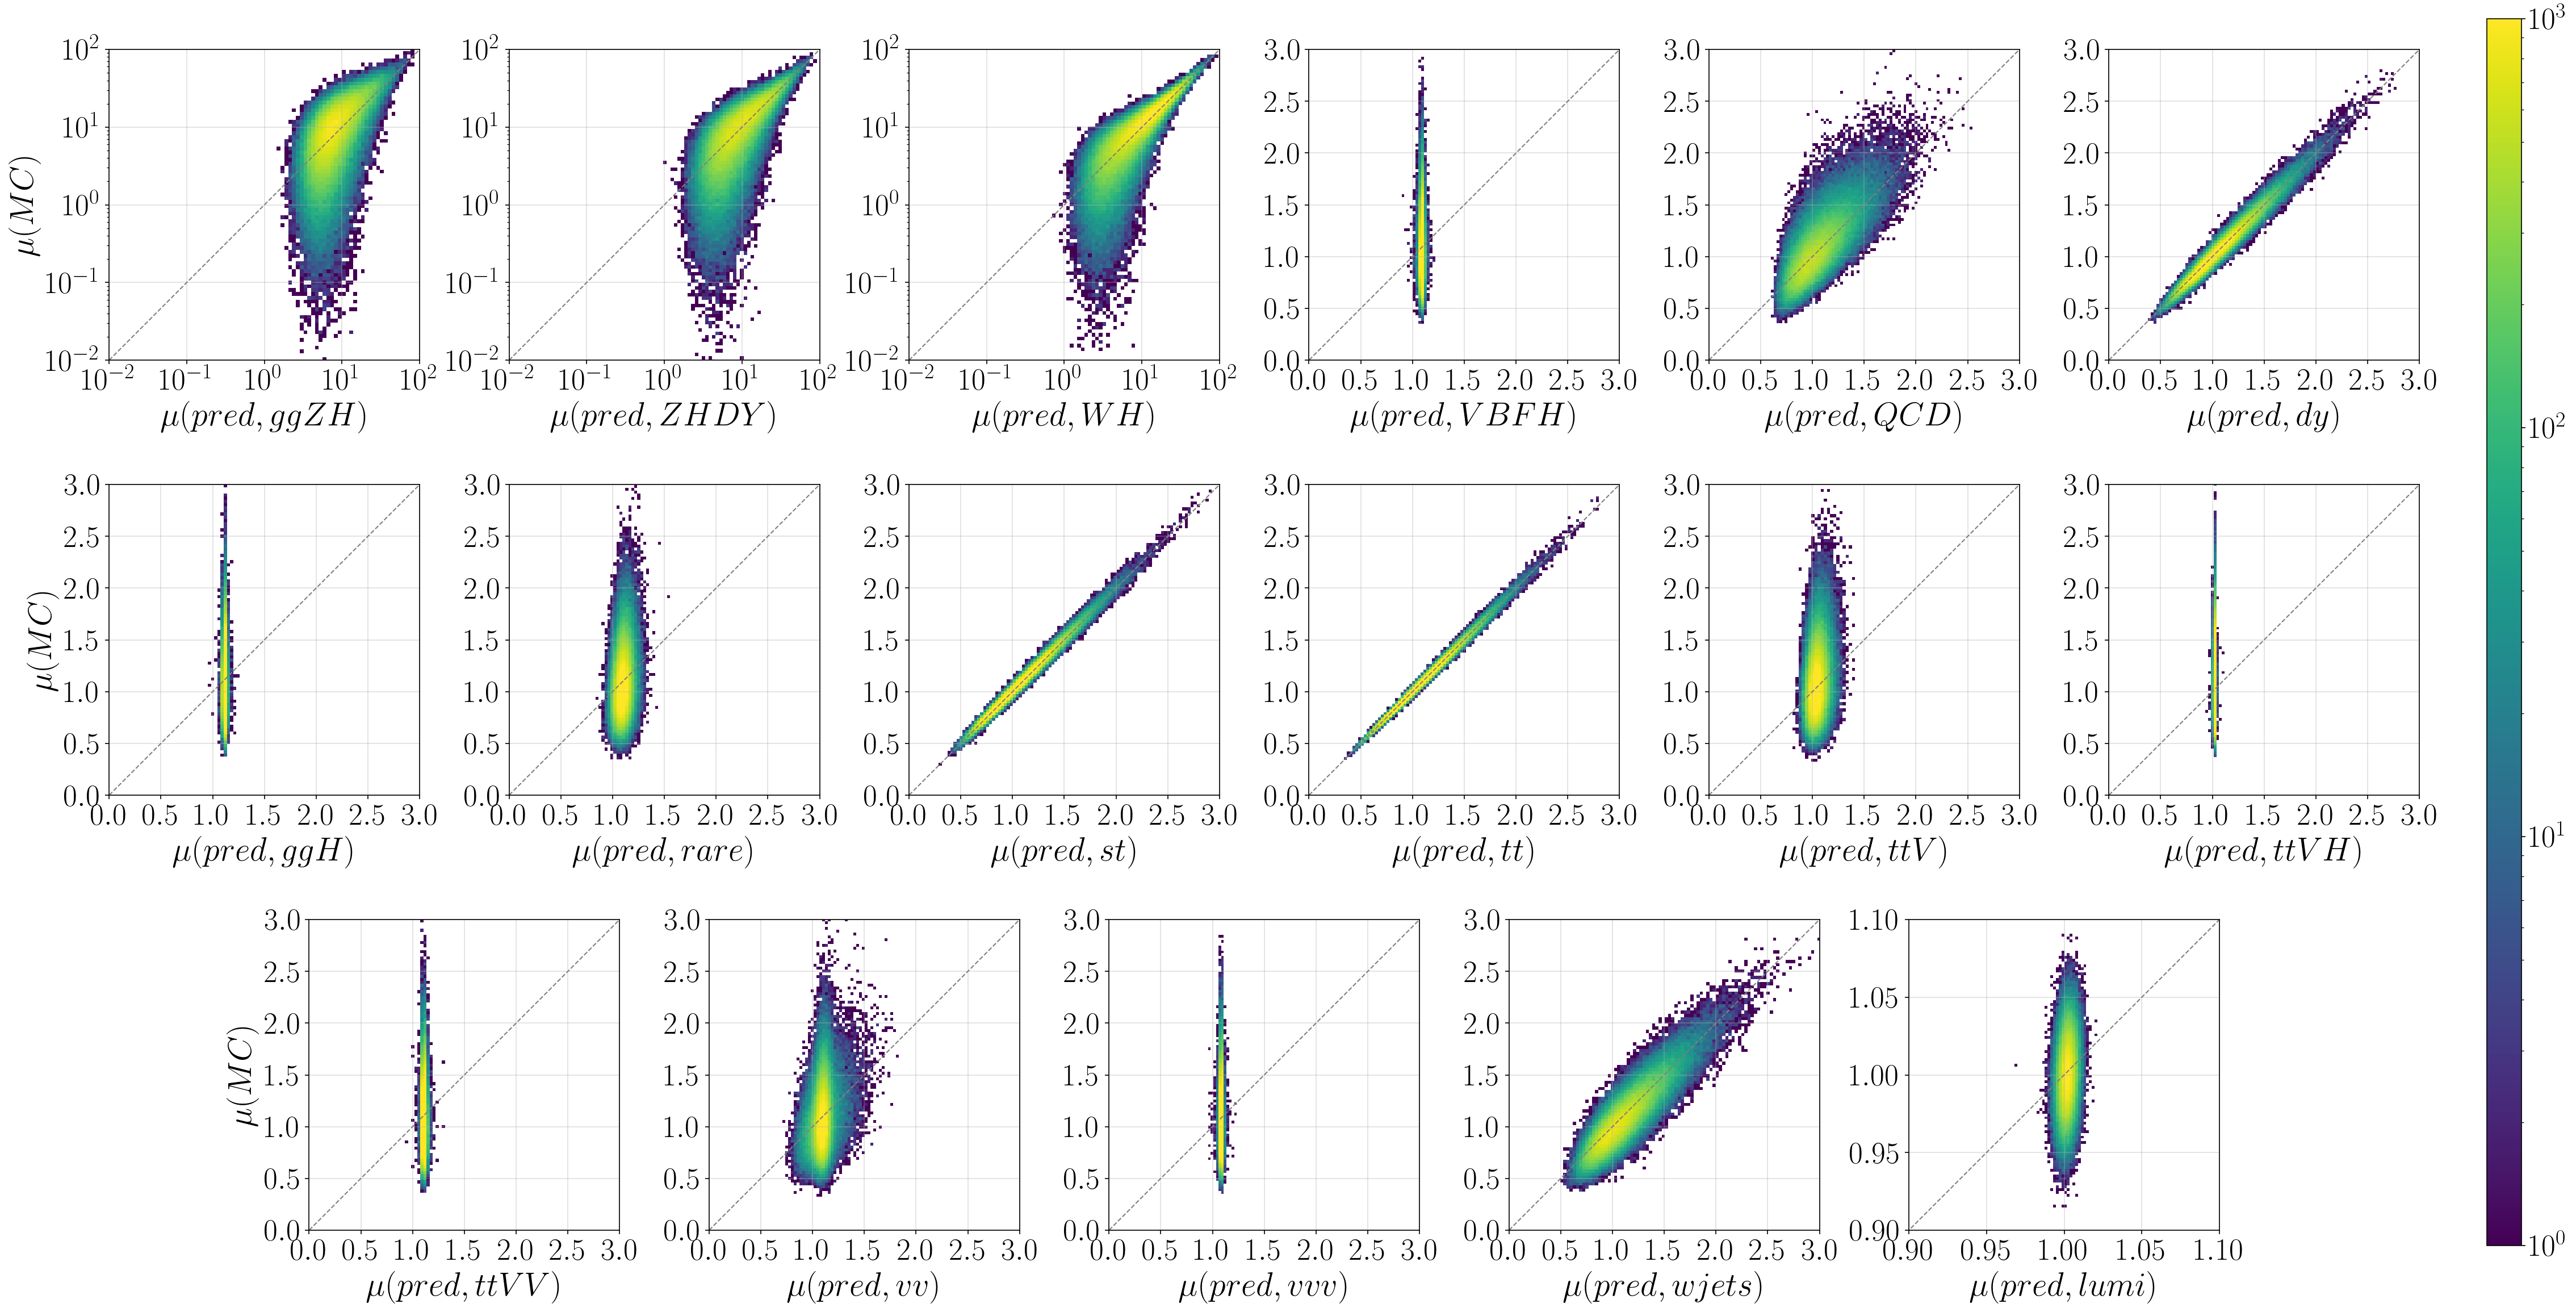
\includegraphics[width=\linewidth]{figures/inference/p_SN}
	\caption{The predicted signal scale parameters vs. the simulated "real" Monte Carlo values. Note the five unrecognized processes, the tail for the signal processes, the well-reconstructed processes and the in-between-quality predictions characterized by the lense-like distribution.}
	\label{fig:predictions}
\end{figure}

The \texttt{WH} process has the highest sensitivity, and the \texttt{ggZH} process the least. In the region $\mu\geq20$ the signal strength modifier parameters are widely and asymmetrically scattered around the perfect predictions in the high-signal region for the $ZH$ processes for both networks. This effect becomes most visible if one switches to linear scales as shown in fig. \ref{fig:predictions_sig_lin}. 

\begin{figure}[h]
	\centering
	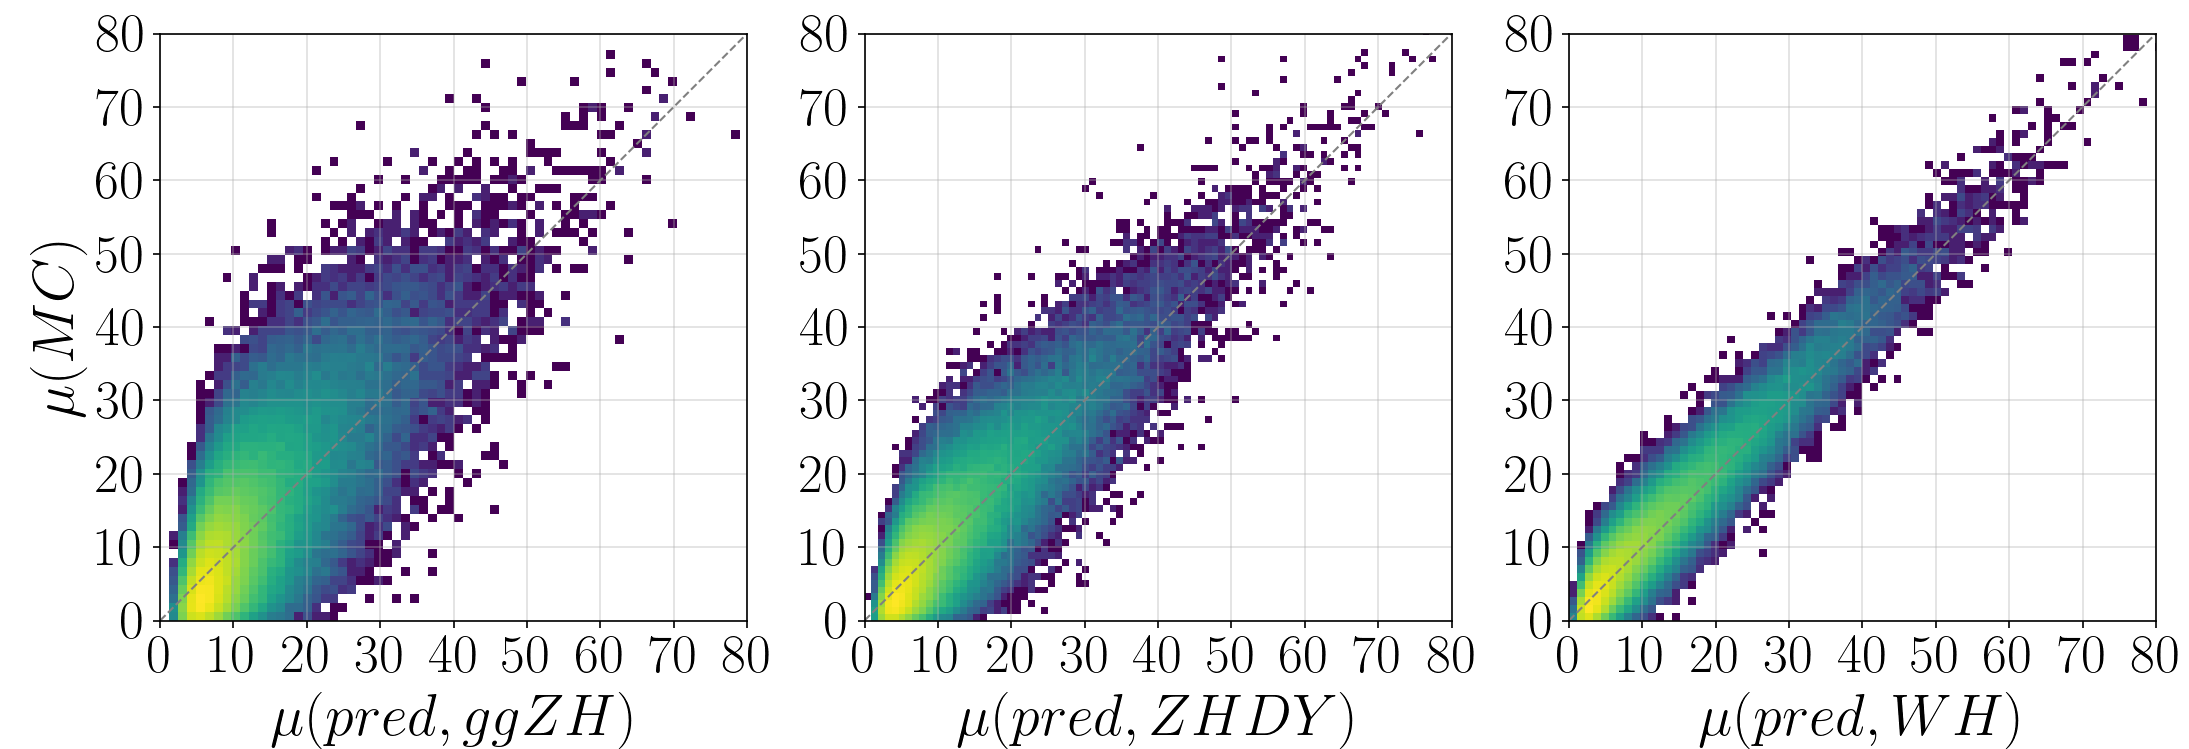
\includegraphics[width=\linewidth]{figures/inference/p_lin}
	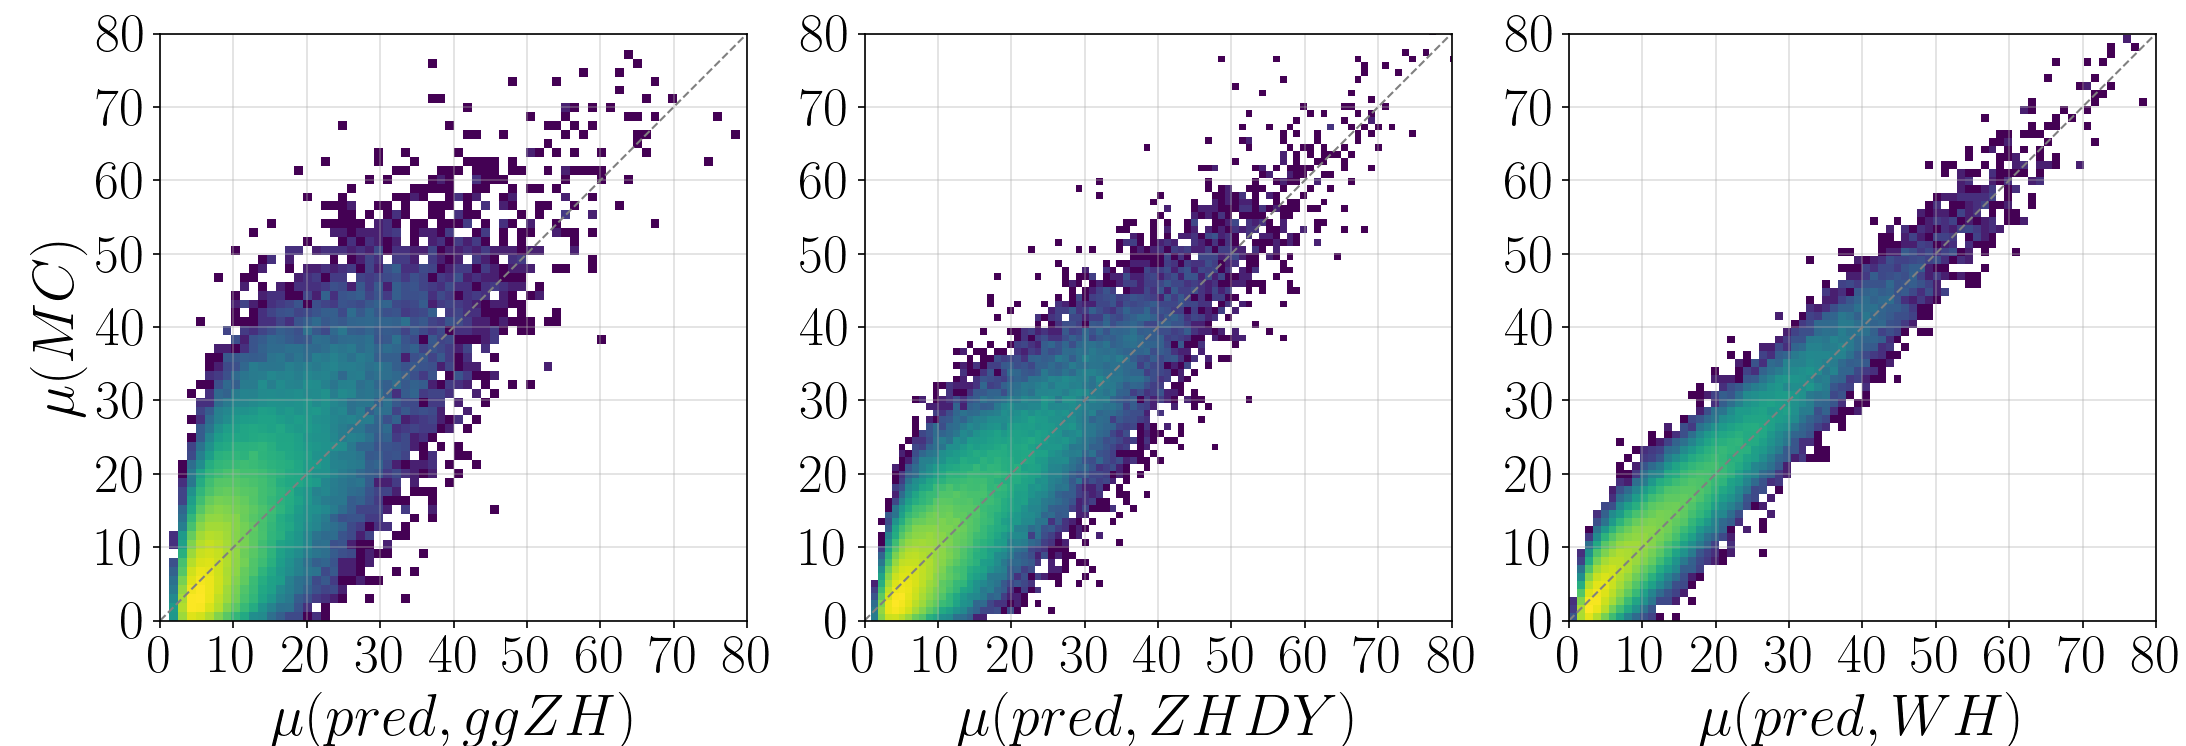
\includegraphics[width=\linewidth]{figures/inference/p_lin_SN}
	\caption{The prediction for the signal processes using a linear axis scale for the cINN (top) and the SN-cINN (bottom). Note the systematic underestimation of the strength modifier parameters most visible for \texttt{ggZH}, \texttt{ZHDY} implying lower sensitivity for these processes.}
	\label{fig:predictions_sig_lin}
\end{figure}

\Subsection{Posterior Inference}

Following the sampling from the target Gaussian function in the latent space, the posteriors can be inferred for the physics parameters for both networks. These are shown in fig. \ref{fig:posteriors} for the nominal histogram where the SM expectation is $\mu=1$. The obtained and normalized posterior distributions are shown in blue. The mean of predicted posterior distribution was taken as prediction, drawn in black. The true values are shown with the red line. The edges of the 68\% quantiles are drawn in blue; these can be interpreted as the uncertainty on the signal strength parameters. The prior distributions for the signal modifier parameters and the nuisance parameters are shown in orange.

\begin{figure}[h!]
	\centering
	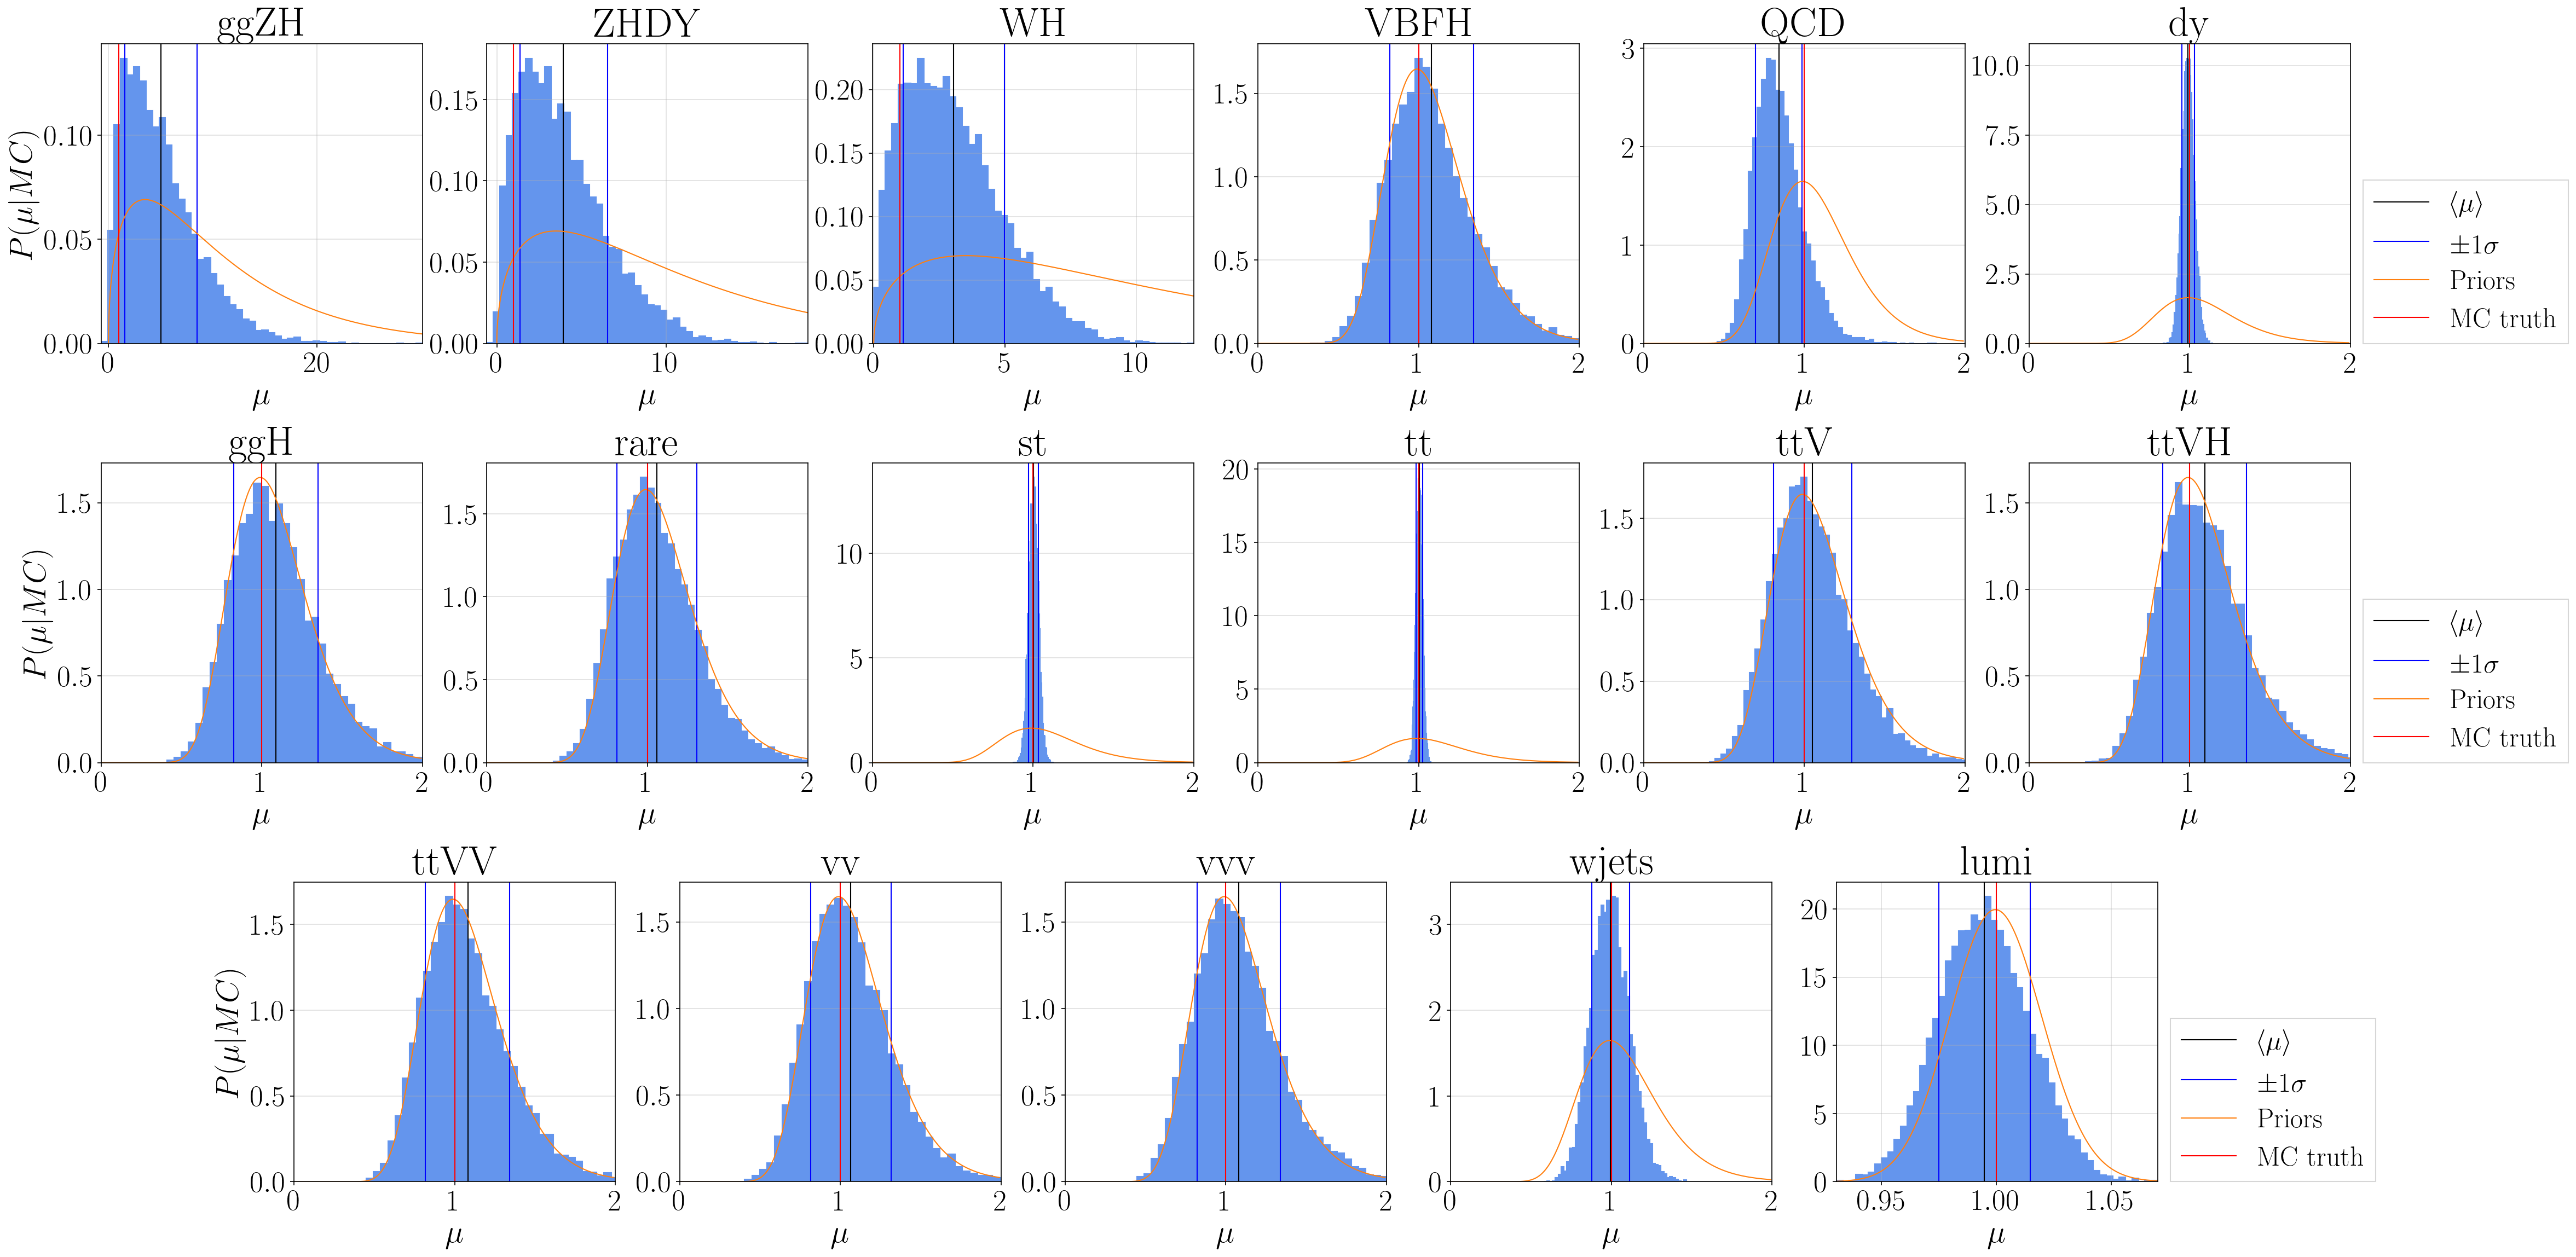
\includegraphics[width=\linewidth]{figures/inference/finalNoSummarye11000_posteriors}
	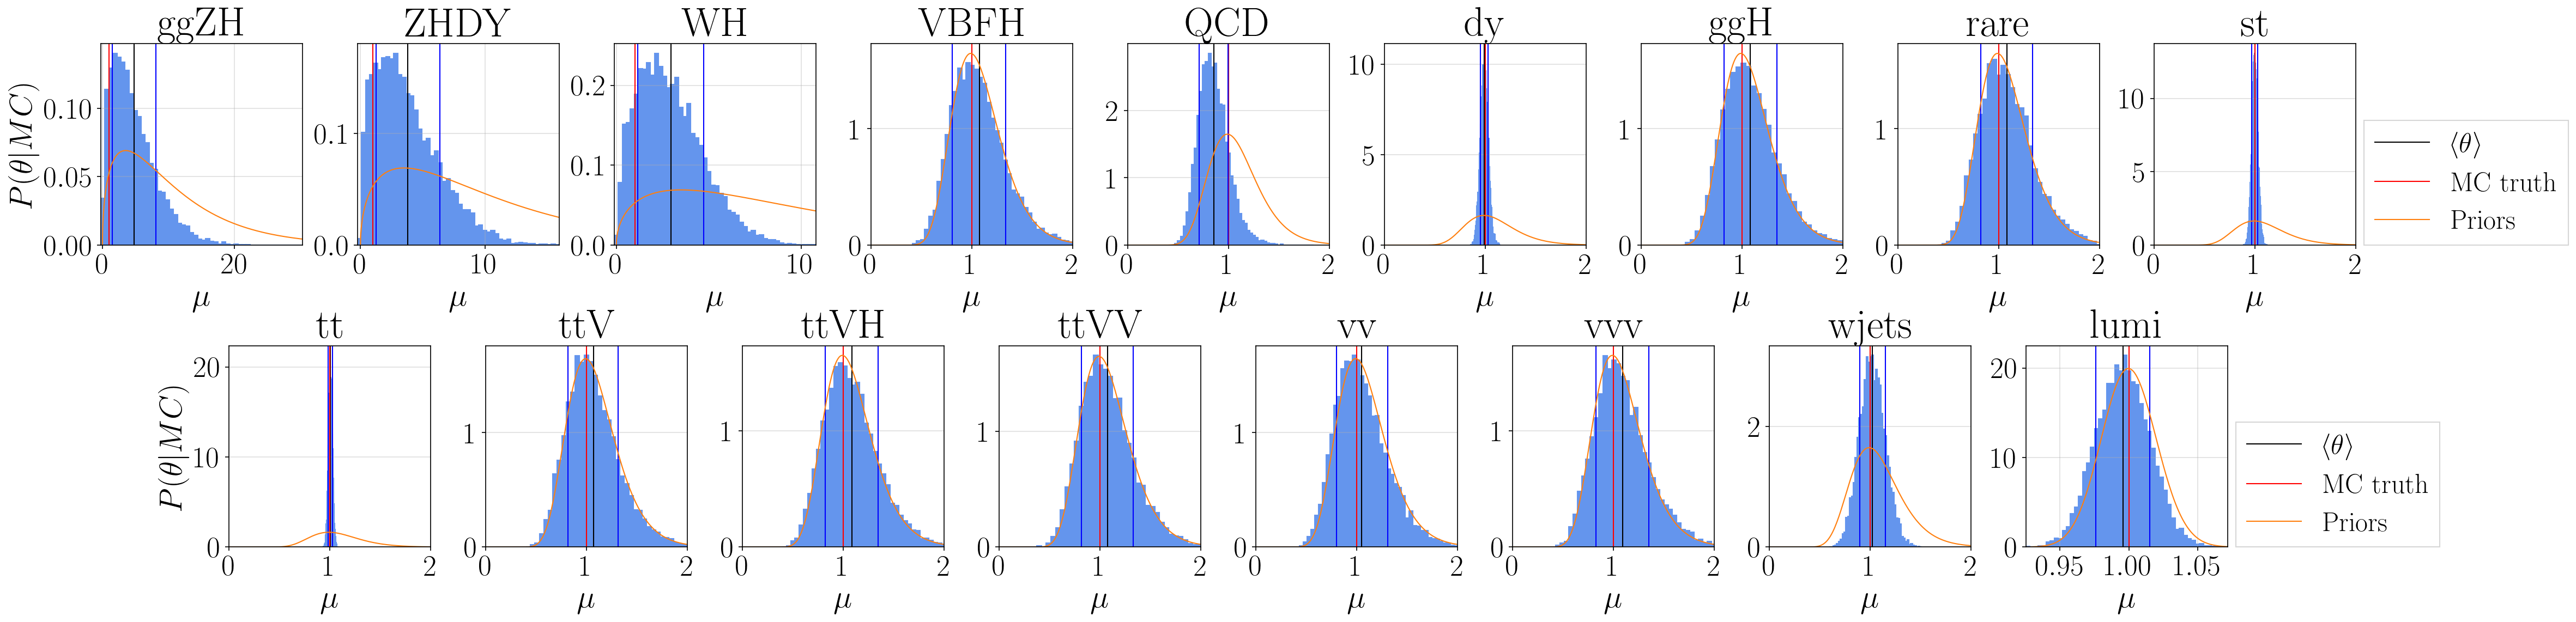
\includegraphics[width=\linewidth]{figures/inference/finalSummary1Layer11000e300NodesCdim100_posteriors}
	\caption{The posterior distributions for each process.}
	\label{fig:posteriors}
\end{figure}

Both networks succeed in the reconstruction of the nominal parameters with differing precision. The networks' sensitivity can be characterized by the width of the posterior distributions for the inferred posteriors. The recognized background processes (\texttt{dy}, \texttt{st}, \texttt{tt}) have an order of magnitude narrower posterior distribution. From the posterior estimation, such behaviour is expected as the calibration curves show no signs of biases, meaning the posteriors should all be scattered around the true values with their widths covering it.

All three signal processes are overestimated with the true values lying closely outside of the 68\% quantiles. All background modifier parameters (except for \texttt{QCD}, which is underestimated and lies outside of the $1\sigma$ range) lie close to their nominal values.

For the weakly recognized and unrecognized processes, especially for the \texttt{VBHF, ggH, rare, ttV, ttVH, ttVV, vv, vvv} processes, the predicted posterior distributions follow the prior distribution closely, as the network has low sensitivity for these parameters. This is also expected from Bayes' Theorem. If some physics observations $y$ are independent of a physics parameter $x$, it means that by Bayes' Theorem the posteriors can be rewritten with the priors $p(x)$ as

\begin{equation*}
	p(x|y) = \frac{p(y|x)p(x)}{p(y)} = \frac{\cancel{p(y)}}{\cancel{p(y)}} p(x).
\end{equation*}

This means the posteriors and the priors coincide. As the independence is mutual, the probability of obtaining $x$ given $y$ does not change either, directly yielding $p(x|y) = p(x)$. Hence, the network returns the prior distribution from one condition only.

In order to study the sensitivity further a small-background high-signal scenario from the test samples has been evaluated and the numerical results for both the SM expectation and this scenario have been summarized in tab. \ref{tab:inference_res}. The posteriors are shown in fig. \ref{fig:HS-SM}. For this scenario the posteriors for \texttt{ZHDY} and \texttt{WH} take a shape of a more symmetric and narrow distribution due to the increased sensitivity as expected. The relative uncertainty has also drastically decreased from $\sim66.54\%$ to $\sim18.19\%$ for \texttt{ZHDY} and from $\sim63.24\%$ to $\sim26.30\%$ for \texttt{WH}. For the third signal process \texttt{ggZH}, this decrease is minor (from $\sim69.22\%$ to $\sim 62.07\%$) due to its small modifier parameter and its lowest share among the three processes. The maximum likelihood fit results from $\texttt{CMSCombine}$ are also shown for comparison. In all cases, the cINN network models have narrower 68\% quantile edges than the fit and the results are compatible within their uncertainties. 

\begin{table}[h!]
	\centering
	\begin{tabular}{ccccccccc}
		\multirow{3}{*}{Processes} & \multicolumn{7}{c}{$\mu$}\\
		&\multicolumn{4}{c}{Nominal}&\multicolumn{4}{c}{High-Signal, Low-Background} \\
%		& \multicolumn{3}{c}{$\mu$} & \multicolumn{2}{c}{$\mu$} \\
		& $\mu^{MC}$ & cINN & SN-cINN & \texttt{CMSCombine} & $\mu^{MC}$ & cINN & SN-cINN & \texttt{CMSCombine} \\[0.1em]
		 \hline\\
		$\mu_\text{ggZH } $ & $1.00$ & $5.10^{+3.57}_{-3.50}$ & $4.86^{+3.38}_{-3.33}$ & $1.00^{+8.16}_{-8.78}$ & $9.01 $ & $10.73^{+6.64}_{-6.68}$ & $10.38^{+6.19}_{-6.18}$ & $9.01^{+9.03}_{-9.40}$\\[0.3em]
		$\mu_\text{ZHDY } $ & $1.00$ & $3.90^{+2.62}_{-2.57}$ & $3.76^{+2.57}_{-2.52}$ & $1.00^{+5.28}_{-5.51}$ & $33.50$ & $35.26^{+5.85}_{-5.89}$ & $36.62^{+6.07}_{-5.98}$ & $33.50^{+6.90}_{-7.30}$ \\[0.3em]
		$\mu_\text{WH   } $ & $1.00$ & $3.02^{+1.92}_{-1.90}$ & $2.93^{+1.80}_{-1.80}$ & $1.00^{+3.44}_{-3.41}$ & $9.95 $ & $11.35^{+2.98}_{-2.99}$ & $11.03^{+2.90}_{-2.93}$ & $9.95^{+3.79}_{-3.62}$ \\[0.3em]
		$\mu_\text{VBFH } $ & $1.00$ & $1.08^{+0.27}_{-0.27}$ & $1.08^{+0.26}_{-0.26}$ & --                        & $0.89 $ & $1.09^{+0.27}_{-0.27}$  & $1.07^{+0.25}_{-0.25}$  & -- \\[0.3em]
		$\mu_\text{QCD  } $ & $1.00$ & $0.84^{+0.14}_{-0.14}$ & $0.86^{+0.15}_{-0.15}$ & --                        & $1.40 $ & $1.17^{+0.18}_{-0.18}$  & $1.12^{+0.17}_{-0.18}$  & -- \\[0.3em]
		$\mu_\text{dy   } $ & $1.00$ & $0.99^{+0.04}_{-0.04}$ & $0.99^{+0.04}_{-0.04}$ & --                        & $1.05 $ & $1.01^{+0.05}_{-0.05}$  & $1.01^{+0.05}_{-0.05}$  & -- \\[0.3em]
		$\mu_\text{ggH  } $ & $1.00$ & $1.09^{+0.27}_{-0.27}$ & $1.08^{+0.26}_{-0.26}$ & --                        & $1.14 $ & $1.09^{+0.27}_{-0.27}$  & $1.08^{+0.25}_{-0.25}$  & -- \\[0.3em]
		$\mu_\text{rare } $ & $1.00$ & $1.06^{+0.25}_{-0.25}$ & $1.08^{+0.26}_{-0.26}$ & --                        & $0.88 $ & $1.03^{+0.23}_{-0.24}$  & $1.10^{+0.27}_{-0.26}$  & -- \\[0.3em]
		$\mu_\text{st   } $ & $1.00$ & $1.00^{+0.03}_{-0.03}$ & $1.00^{+0.03}_{-0.03}$ & --                        & $0.84 $ & $0.78^{+0.03}_{-0.03}$  & $0.77^{+0.03}_{-0.03}$  & -- \\[0.3em]
		$\mu_\text{tt   } $ & $1.00$ & $1.00^{+0.02}_{-0.02}$ & $1.00^{+0.02}_{-0.02}$ & --                        & $0.79 $ & $0.78^{+0.02}_{-0.02}$  & $0.78^{+0.02}_{-0.02}$  & -- \\[0.3em]
		$\mu_\text{ttV  } $ & $1.00$ & $1.05^{+0.24}_{-0.24}$ & $1.07^{+0.25}_{-0.25}$ & --                        & $0.52 $ & $1.02^{+0.23}_{-0.23}$  & $1.05^{+0.24}_{-0.24}$  & -- \\[0.3em]
		$\mu_\text{ttVH } $ & $1.00$ & $1.09^{+0.27}_{-0.27}$ & $1.08^{+0.27}_{-0.27}$ & --                        & $0.96 $ & $1.08^{+0.26}_{-0.26}$  & $1.07^{+0.26}_{-0.26}$  & -- \\[0.3em]
		$\mu_\text{ttVV } $ & $1.00$ & $1.08^{+0.26}_{-0.27}$ & $1.07^{+0.26}_{-0.26}$ & --                        & $0.69 $ & $1.08^{+0.27}_{-0.27}$  & $1.08^{+0.25}_{-0.25}$  & -- \\[0.3em]
		$\mu_\text{vv   } $ & $1.00$ & $1.06^{+0.25}_{-0.25}$ & $1.06^{+0.25}_{-0.25}$ & --                        & $1.43 $ & $1.18^{+0.29}_{-0.30}$  & $1.21^{+0.30}_{-0.30}$  & -- \\[0.3em]
		$\mu_\text{vvv  } $ & $1.00$ & $1.09^{+0.27}_{-0.27}$ & $1.09^{+0.27}_{-0.27}$ & --                        & $0.84 $ & $1.09^{+0.26}_{-0.27}$  & $1.07^{+0.25}_{-0.26}$  & -- \\[0.3em]
		$\mu_\text{wjets} $ & $1.00$ & $0.99^{+0.12}_{-0.12}$ & $1.02^{+0.13}_{-0.13}$ & --                        & $1.05 $ & $1.17^{+0.12}_{-0.13}$  & $1.22^{+0.13}_{-0.13}$  & -- \\[0.3em]
		$\mu_\text{lumi } $ & $1.00$ & $1.00^{+0.02}_{-0.02}$ & $1.00^{+0.02}_{-0.02}$ & --                        & $0.98 $ & $1.00^{+0.02}_{-0.02}$  & $1.00^{+0.02}_{-0.02}$  & -- \\[0.3em]
		\hline
	\end{tabular}
	\caption{The predicted values of the signal strength modifier and of the nuisance parameters for the cINN and the summary-network extended network (SN-cINN) for the nominal and the high-signal, low-background scenario. For comparison, the likelihood fit result is indicated.}
	\label{tab:inference_res}
\end{table}

\begin{figure}[h!]
	\centering
	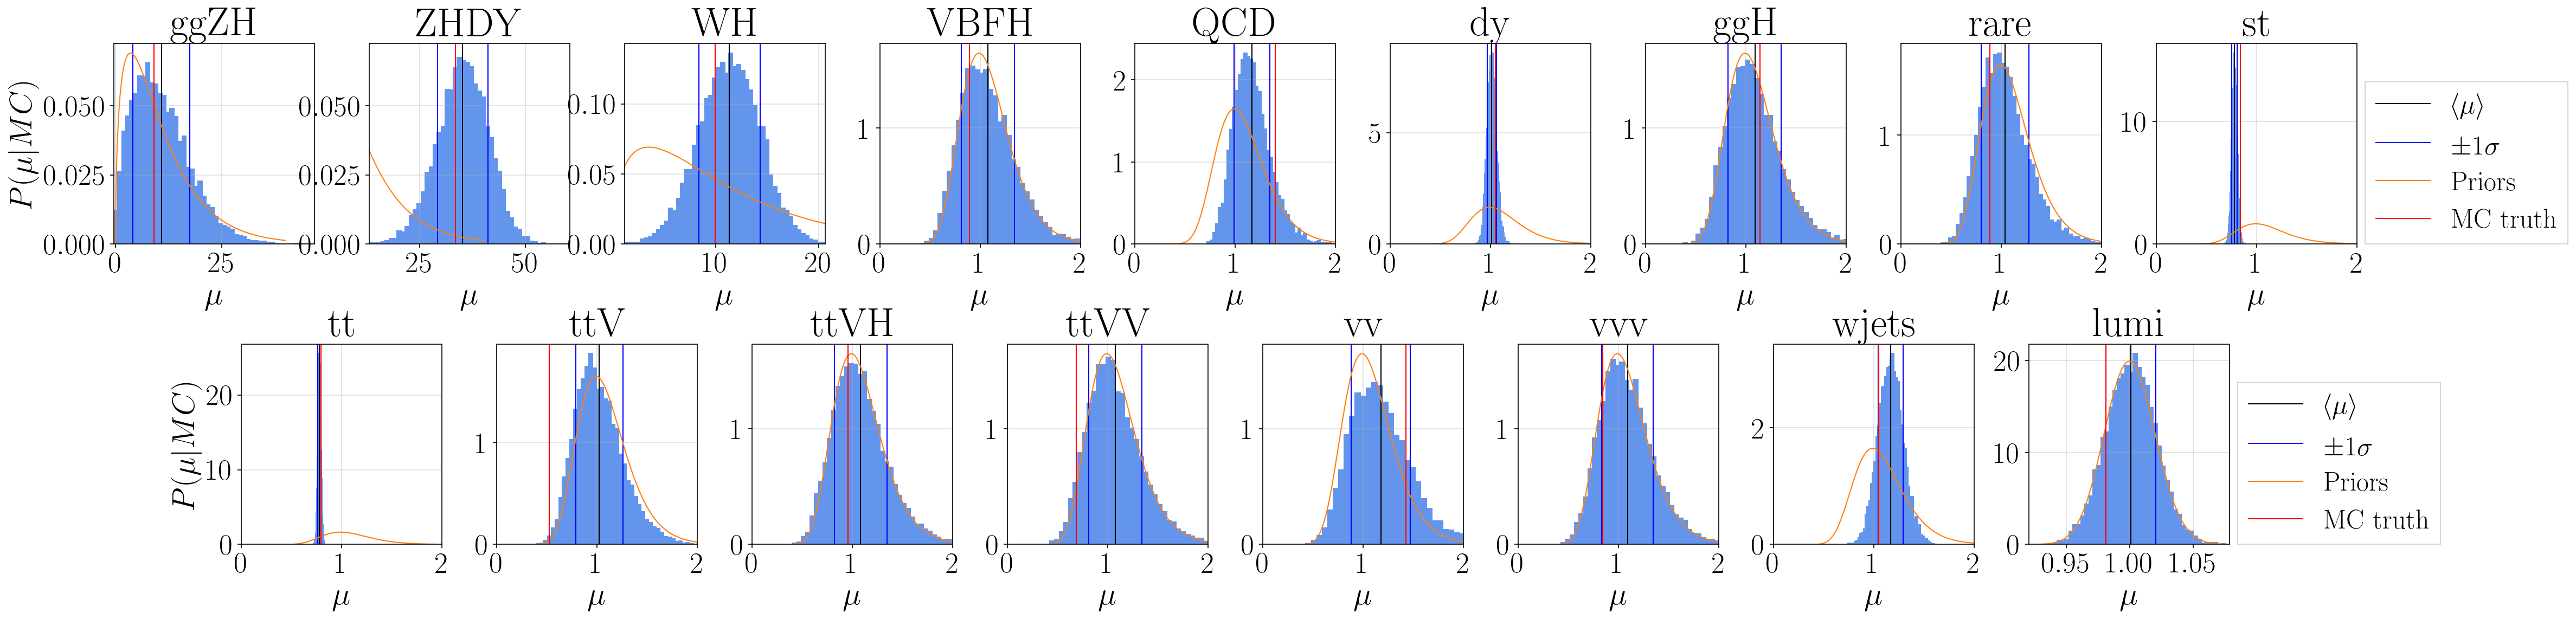
\includegraphics[width=\linewidth]{figures/inference/194finalNoSummarye11000_posteriors}
	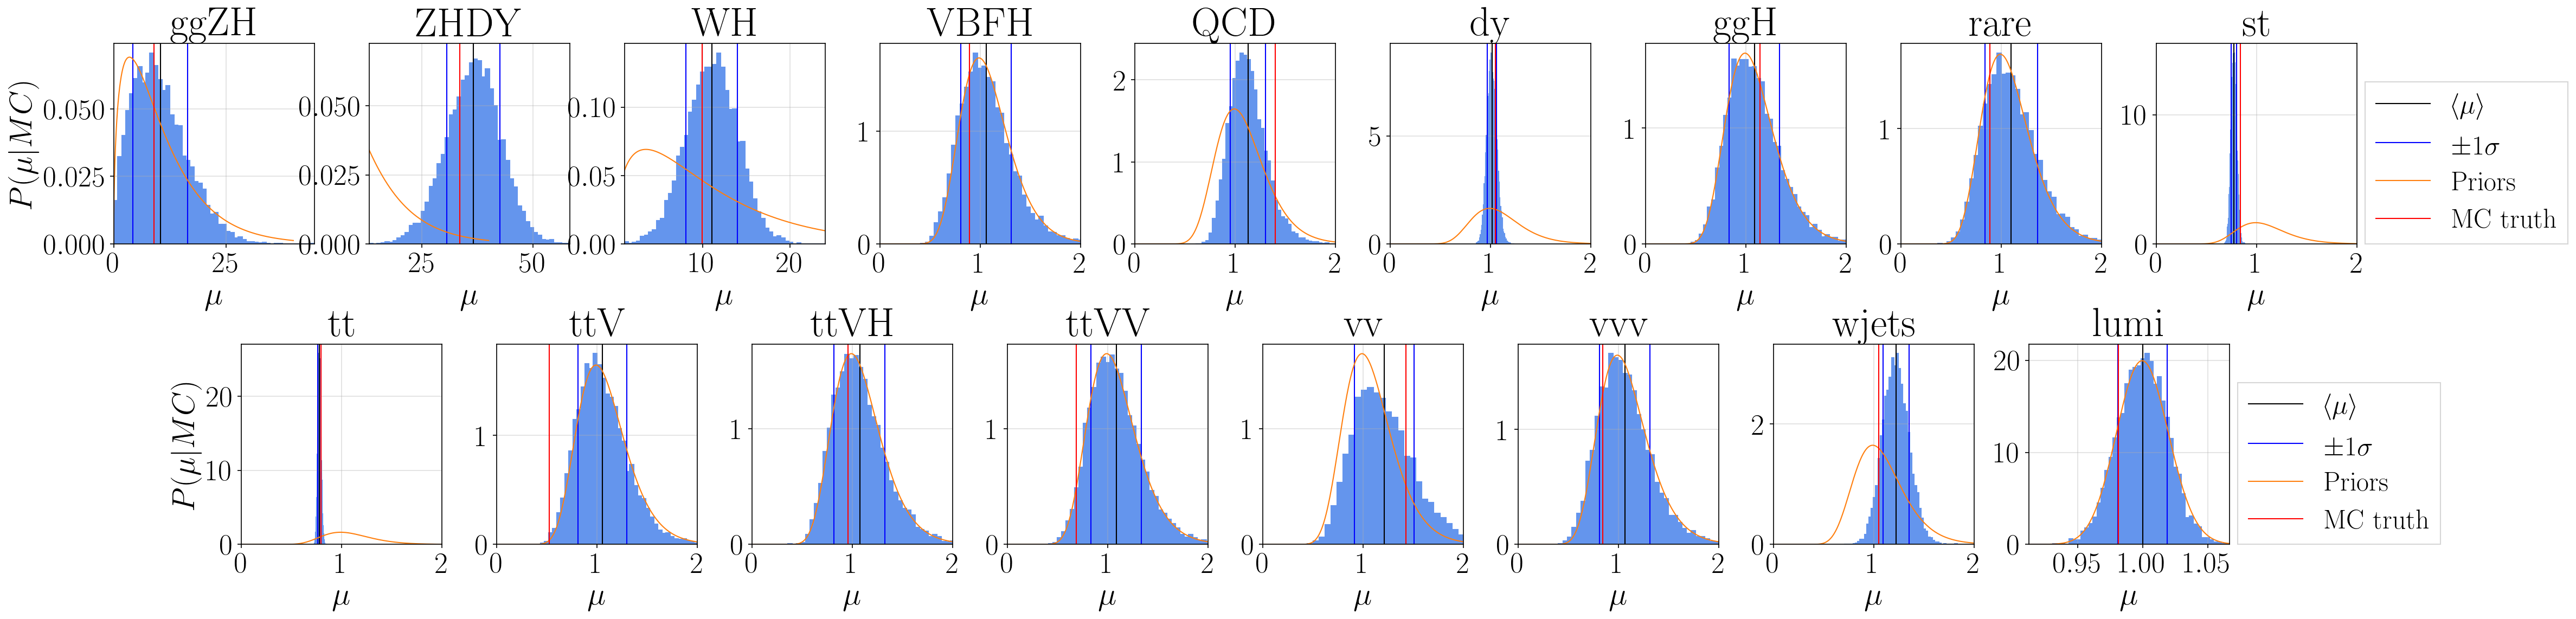
\includegraphics[width=\linewidth]{figures/inference/194finalSummary1Layer11000e300NodesCdim100_posteriors}
	\caption{Posterior distributions for the selected high-signal small-background scenario. Note the more symmetric shape of the signal distributions and the thinner posterior distribution relative to the MC expected value showing increased network sensitivity. For the unrecognized processes, their posterior distribution is reproduced.}
	\label{fig:HS-SM}
\end{figure}

According to the prediction distributions and to the posteriors the luminosity nuisance parameter can be considered as a weakly recognized parameter due the lens-like shape of the former and the minimal shape changes (compared to prior) in the latter. As it acts as a normalizing uncertainty scaling the integral of the histogram -- hence every bin altogether -- it is not surprising the network has difficulties reconstructing them correctly due to the other occurring shape-changing and normalizing nuisance parameters inherent in the conditions.

It occurs that the SN-cINN and the cINN can both reproduce the same results under similar conditions. The SN-cINN carries unfortunately two intrinsic conceptual disadvantages: first, it reduces the input dimension of the physics observable and second, it is often prone to overtraining empirically. Naïvely, the reduction and reweighing of the conditions should benefit the training; however, the bins in the condition histogram are independent of each other and this reweighing can be then performed by the subnetworks in the GLOW blocks themselves. In other words, any reduction in dimensionality by the summary network itself in case of uncorrelated data yields implicit information loss reducing training performance. This is also reflected by the lack of "network architecture flexibility": forcing the SN-cINN architectures requires a lot of arbitrary fine-tuning per hand and only some individual setups are stable. For this reason, the cINN setup is superior compared to the SN-cINN setup for this specific case.